\documentclass[10pt, a4paper]{article}

\usepackage[utf8]{inputenc}
\usepackage[english,spanish]{babel}
\usepackage[left=25mm, right=25mm, top=35mm, bottom=30mm, headheight=35mm]{geometry}
\usepackage{graphicx}
\usepackage{xcolor}
\usepackage{fancyhdr}
\usepackage{hyperref}
\usepackage{setspace}
\usepackage{float}
\usepackage{listings}
\lstset{
  basicstyle=\ttfamily,
  keywordstyle=\color{blue},
  commentstyle=\color{green},
  stringstyle=\color{red},
  showstringspaces=false,
  breaklines=true,
  frame=single,
  backgroundcolor=\color{lightgray},
  columns=fullflexible
}
\lstdefinestyle{JavaStyle}{
    language=Java,
    basicstyle=\small\ttfamily,
    keywordstyle=\color{blue},
    commentstyle=\color{green},
    stringstyle=\color{purple},
    tabsize=4,
    showspaces=false,
    showstringspaces=false
} 
\lstdefinestyle{JavaScriptStyle}{
    language=JavaScript,
    basicstyle=\small\ttfamily,
    keywordstyle=\color{blue},
    commentstyle=\color{green},
    stringstyle=\color{purple},
    tabsize=4,
    showspaces=false,
    showstringspaces=false
} 

% Define background color
\definecolor{background}{HTML}{2E3440}

% Syntax customization
\usepackage{minted}
\usemintedstyle{nord}
\setminted{bgcolor=background}
\setminted{breaklines}

% Variables
\newcommand{\university}{Universidad Nacional de San Agustín de Arequipa}
\newcommand{\faculty}{Facultad de Ingeniería de Producción y Servicios}
\newcommand{\program}{Escuela Profesional de Ingeniería de Sistemas}
\newcommand{\semester}{2024 - A}
\newcommand{\course}{img/web_programming}
\newcommand{\topic}{img/Django.jpg} 
\newcommand{\professor}{Carlo Jose Luis Corrales Delgado}
\newcommand{\students}{Mamani Anahua, Victor Narciso} 
\newcommand{\github}{https://github.com/VictorMA18/Lab07-Django-Telusko}
\newcommand{\video}{}
\newcommand{\mydate}{5 de junio, 2024}

% Just parts and chapters numbered
\setcounter{secnumdepth}{0}

% Head and foot customization
\pagestyle{fancy}
\lhead{\raisebox{-0.2\height}{
\includegraphics[width=4cm]{img/logo_unsa.png}}}
\chead{\fontsize{8}{8}\selectfont \university \\ \faculty \\ \textbf{\program}}
\rhead{\raisebox{-0.2\height}{
\includegraphics[width=3.5cm]{img/logo_episunsa.png}}}
% \lfoot{Estudiante \student}
\lfoot{Semestre \semester}
\cfoot{}
\rfoot{Pág. \thepage}

\begin{document}

\begin{titlepage}
	\centering
	\includegraphics[width=14cm]{\course} \par
  \vfill \vfill
	\includegraphics[width=15cm]{\topic}\par
  \vfill \vfill
  {\textbf{Profesor(a):} \par}
	\professor \vfill
  {\textbf{Estudiantes:} \par}
	\students \vfill
  {\textbf{Repositorio GitHub:} \par}
  \href{\github}{\github} \vfill
  {\textbf{Video:} \par}
  \href{\video}{\video} \vfill
	{\large \mydate \par}
\end{titlepage}

\section{TRAVELLO}

\section{Clases en Models.py}
Este código define un modelo en Django llamado Destination, que representa un destino turístico. Cada destino tiene un nombre, una imagen, una descripción, un precio y un indicador de oferta. El nombre se almacena como texto, la imagen se guarda en un directorio específico, la descripción es un texto largo, el precio es un número entero, y la oferta es un valor booleano que indica si hay una oferta especial para ese destino.
\begin{figure}[H]
  \centering
  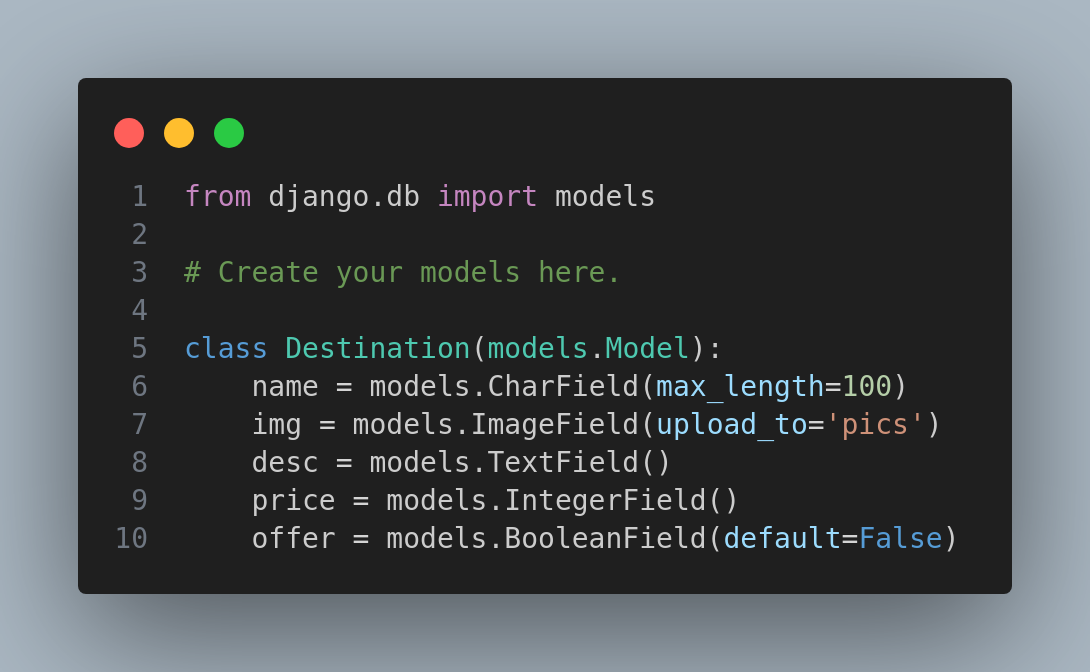
\includegraphics[width=0.7\textwidth]{img/models-travello.png}
  \caption{Codigo y Ejecucion}
\end{figure}

\section{Funciones en Views.py}
Este código define una vista en Django que renderiza una plantilla HTML llamada index.html. La vista obtiene todos los objetos Destination del modelo y los pasa a la plantilla como contexto, bajo el nombre dests. Cuando un usuario accede a la página asociada a esta vista, verá una lista de destinos turísticos que se han recuperado de la base de datos.

\begin{figure}[H]
  \centering
  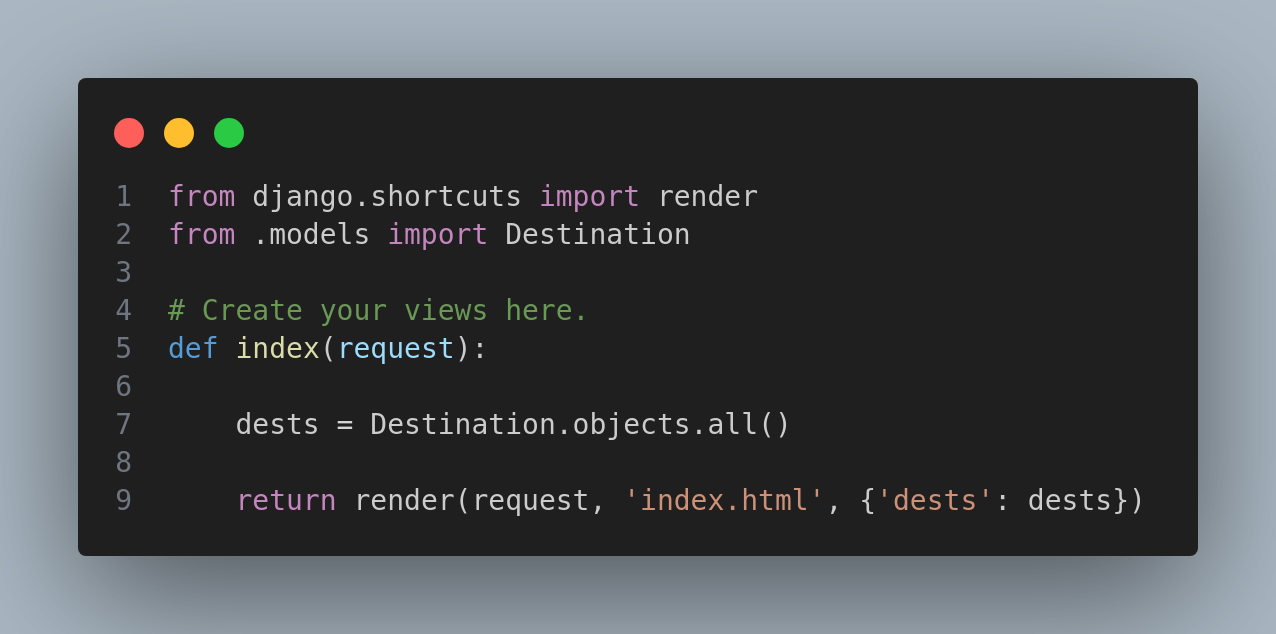
\includegraphics[width=0.7\textwidth]{img/views-travello.png}
  \caption{Codigo y Ejecucion}
\end{figure}

\section{Funciones en Urls.py}
Este archivo define las URL para la aplicación Django. La URL vacía ('') está asociada a la vista index definida en el archivo views.py de la misma aplicación. Cuando un usuario visita la página principal del sitio, se llama a la función index en views.py, que renderiza la plantilla index.html.}

\begin{figure}[H]
  \centering
  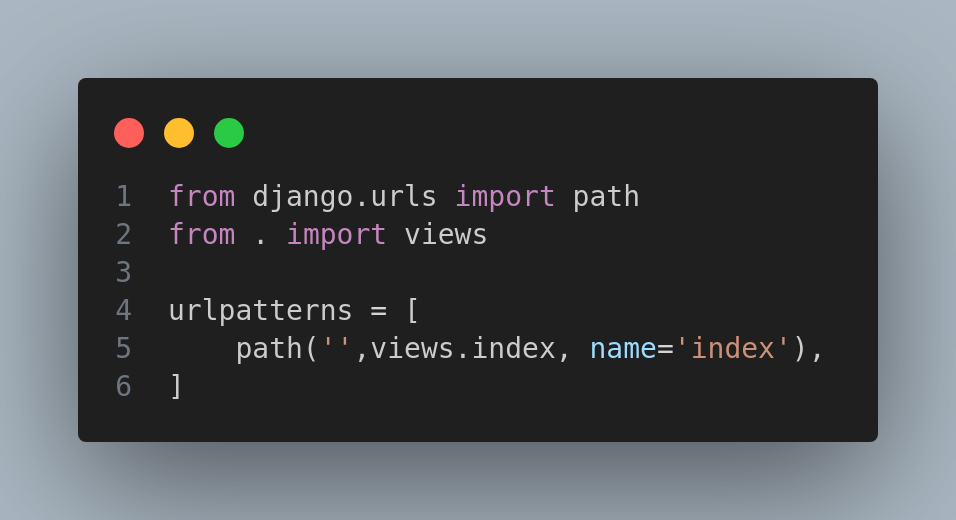
\includegraphics[width=0.7\textwidth]{img/urls-travello.png}
  \caption{Codigo y Ejecucion}
\end{figure}

\section{Funciones en Admin.py}
En este código, se importa la clase Destination del archivo models.py de la misma aplicación Django. Luego, esta clase se registra en el panel de administración de Django utilizando admin.site.register(), lo que permite administrar los objetos de esta clase directamente desde el panel de administración. Esto facilita la gestión de los datos del modelo Destination a través de la interfaz de administración de Django.
\begin{figure}[H]
  \centering
  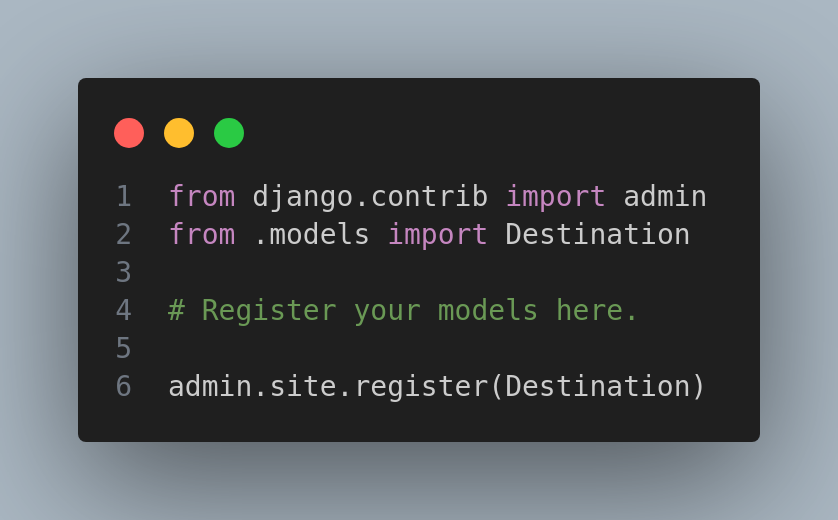
\includegraphics[width=0.7\textwidth]{img/admin-travello.png}
  \caption{Codigo y Ejecucion}
\end{figure}

\section{Los archivos HTML}
Para poder visualizar el index nos ponemos en
travello \href{http://127.0.0.1:8000}{http://127.0.0.1:8000}

\begin{figure}[H]
  \centering
  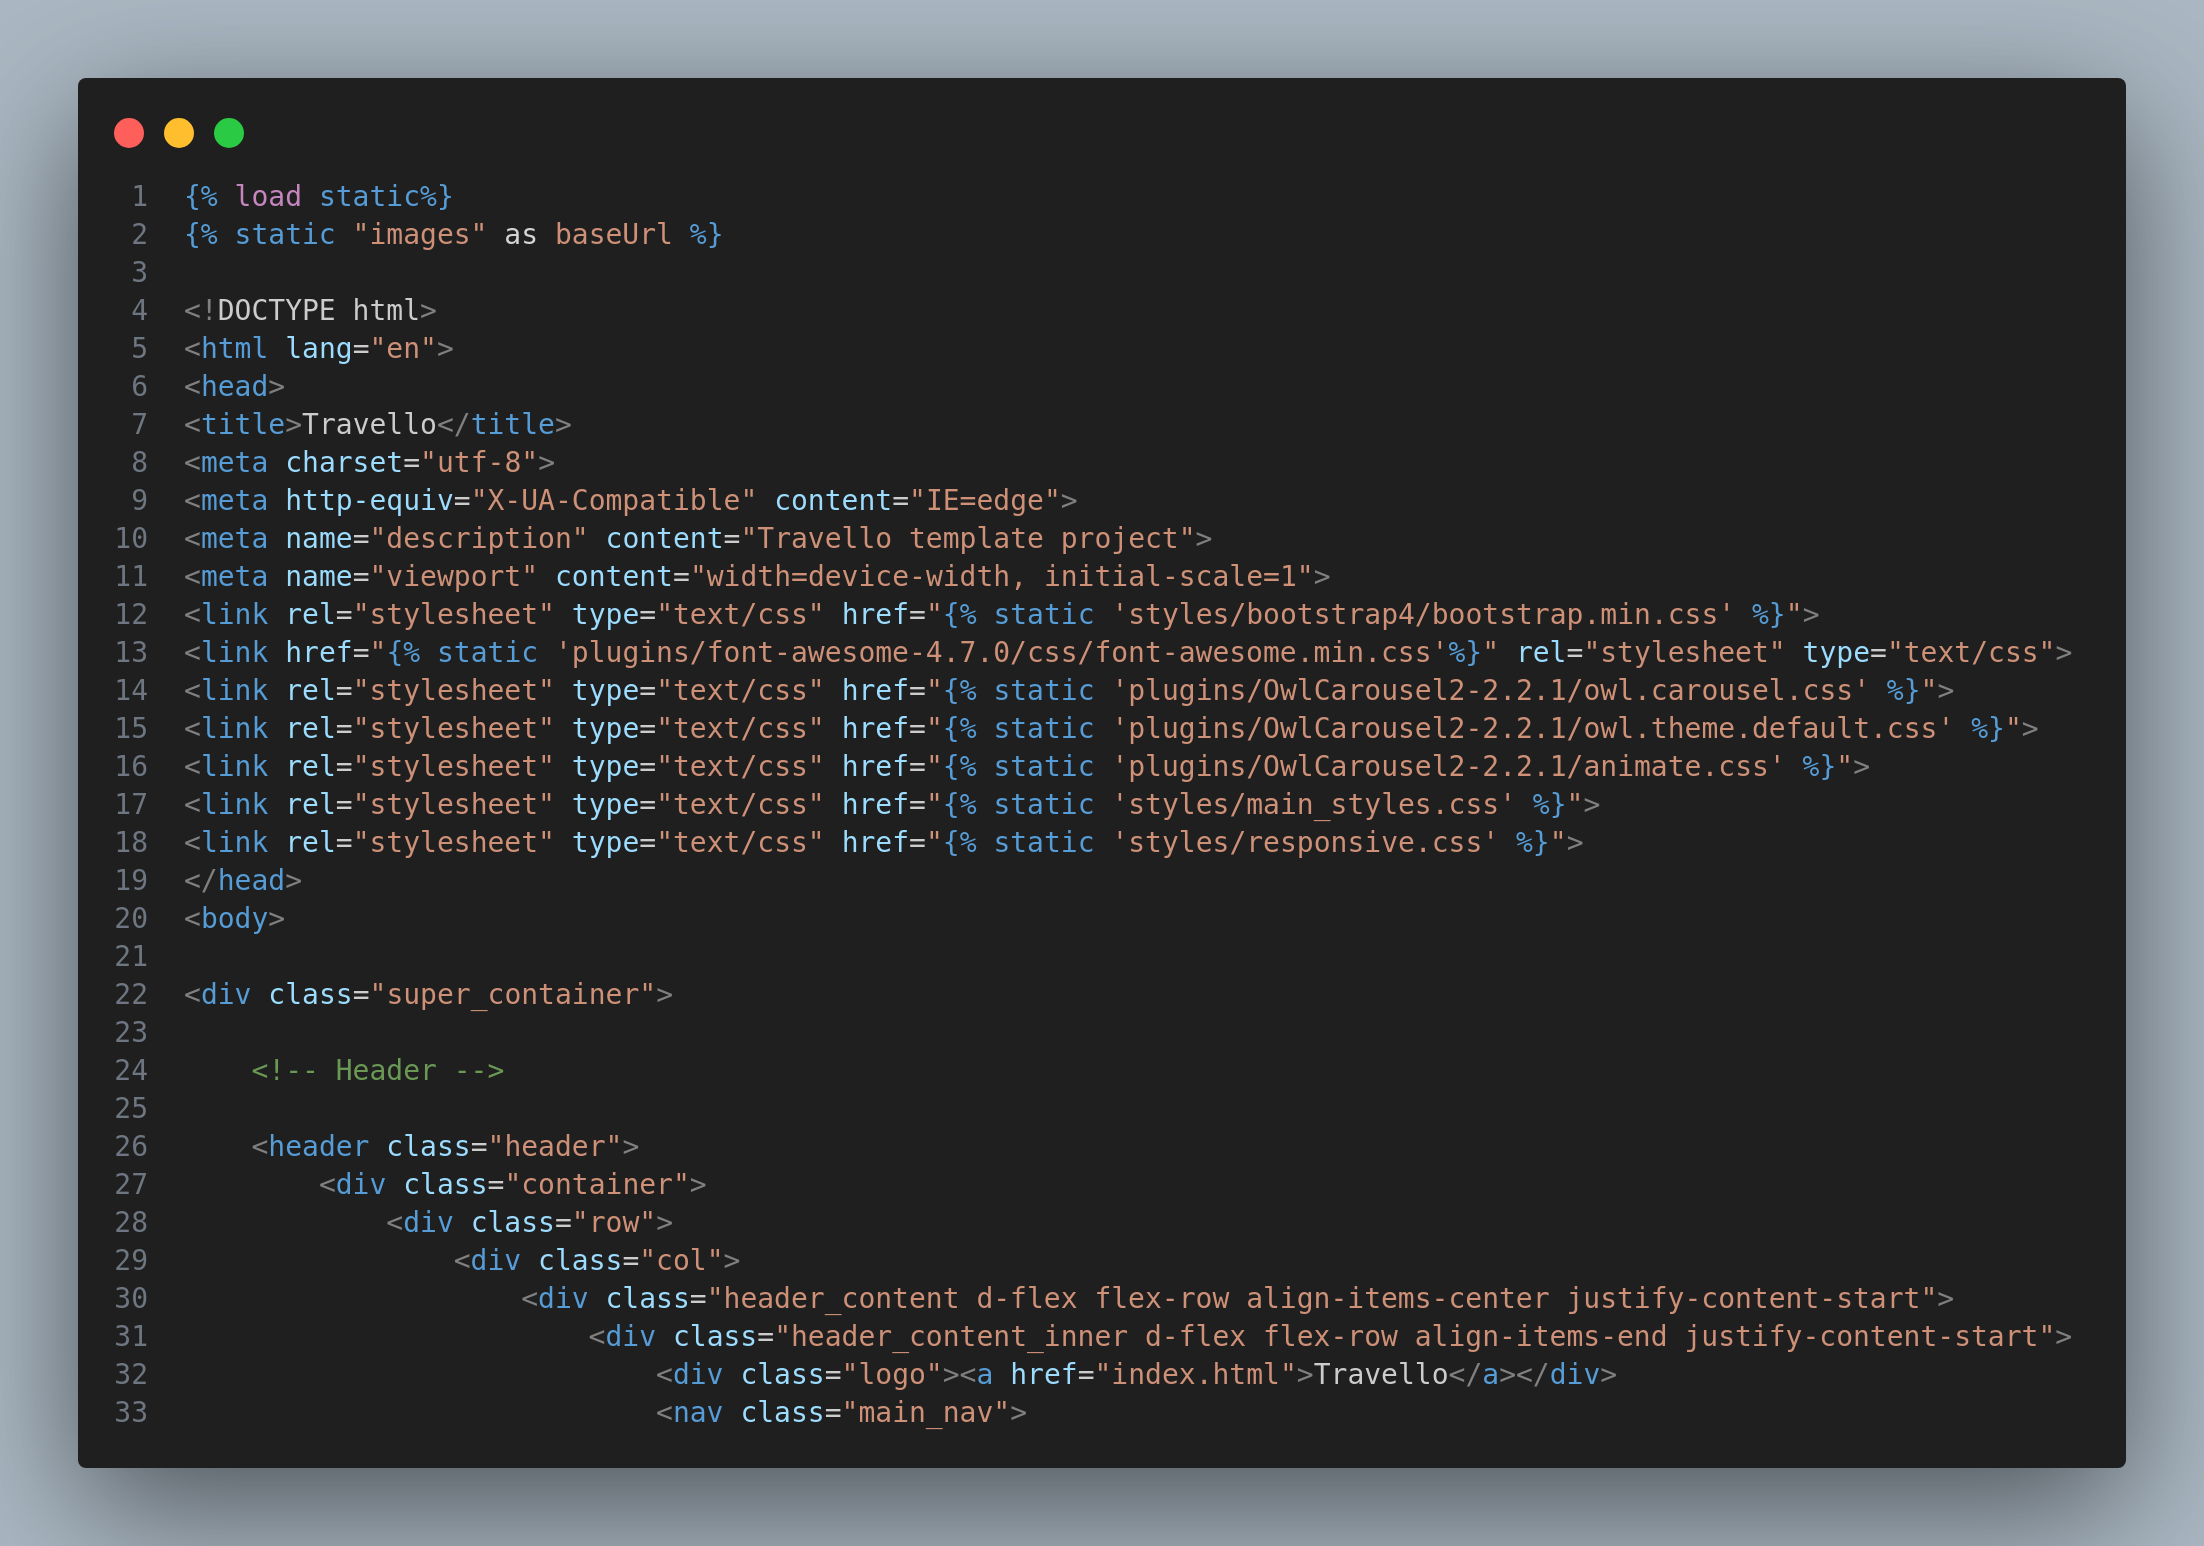
\includegraphics[width=0.7\textwidth]{img/index-html.png}
  \caption{Codigo y Ejecucion}
\end{figure}

\begin{figure}[H]
  \centering
  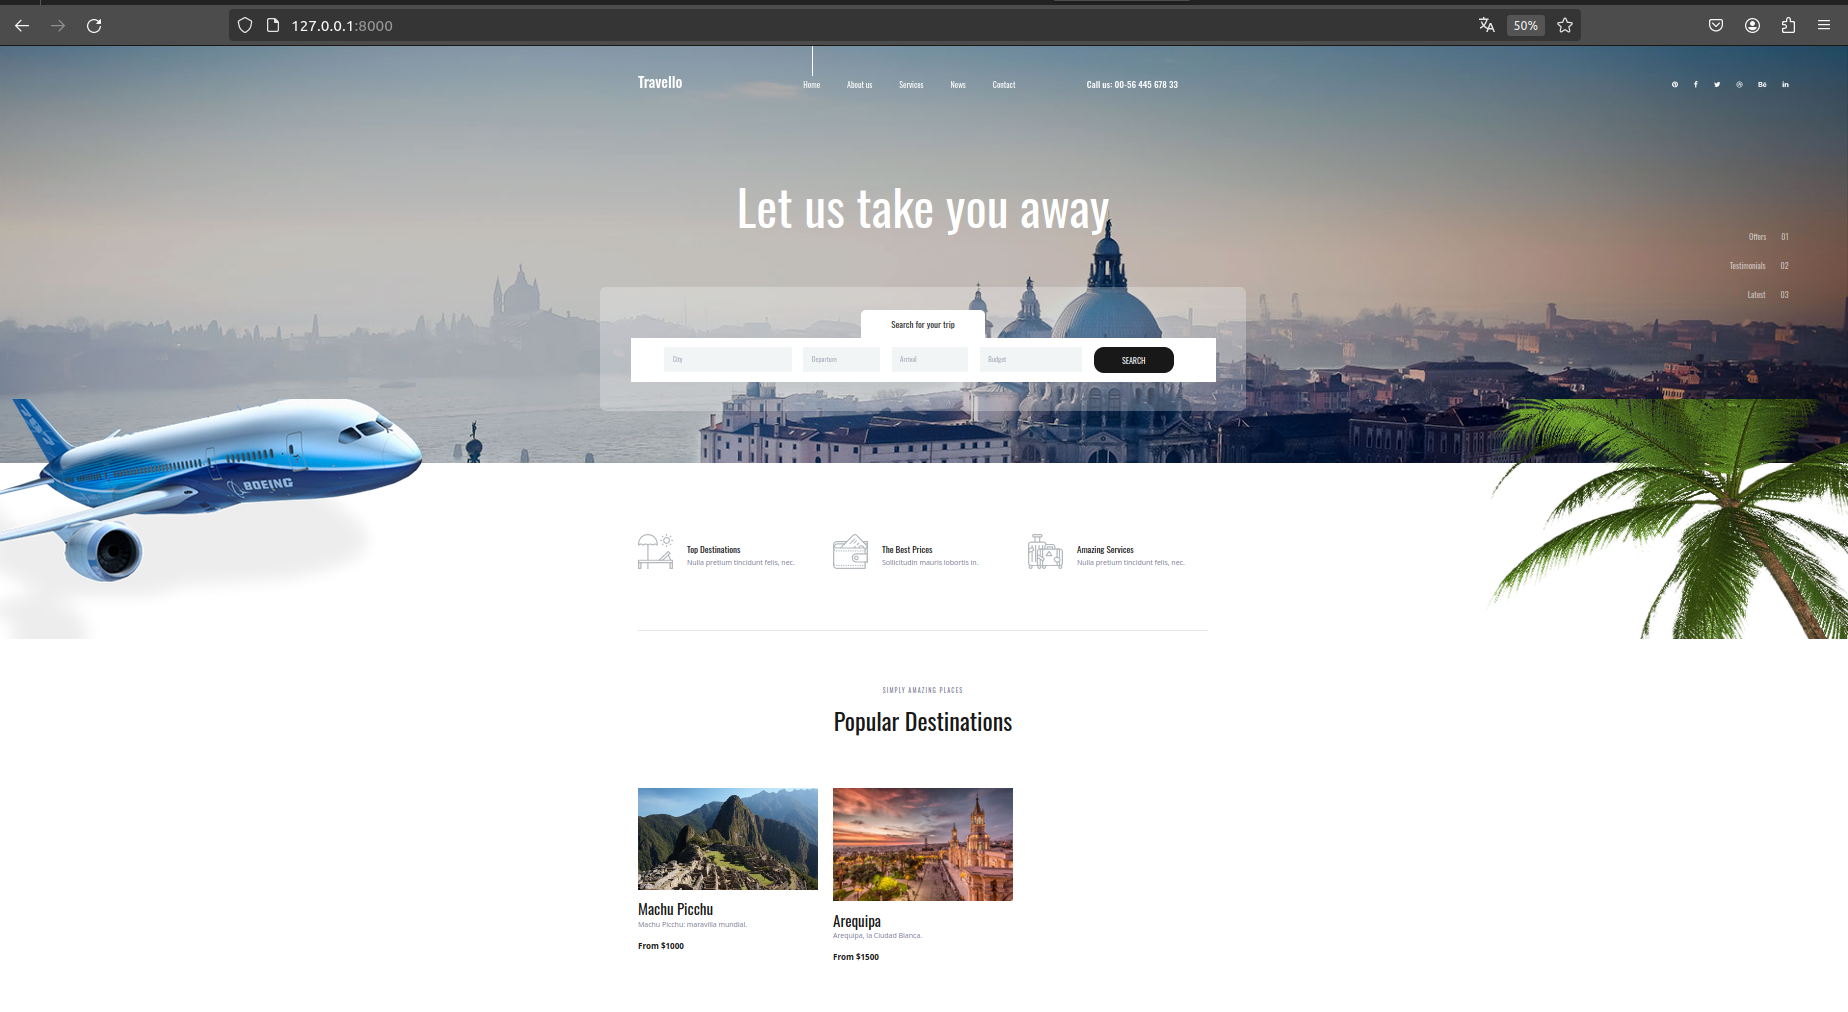
\includegraphics[width=0.7\textwidth]{img/index.png}
  \caption{Codigo y Ejecucion}
\end{figure}

\section{Base de Datos PostgradeSQL}

\section{Entrar a Django Admin}
Crear un destino en \href{http://127.0.0.1:8000/admin/login/?next=/admin/}{http://127.0.0.1:8000/admin/login/?next=/admin/}
\singlespacing
Cuando entremos hay que crear un superusuario para el admin y poder administrar la base de datos para esto hay crearlo desde la terminal

\begin{figure}[H]
  \centering
  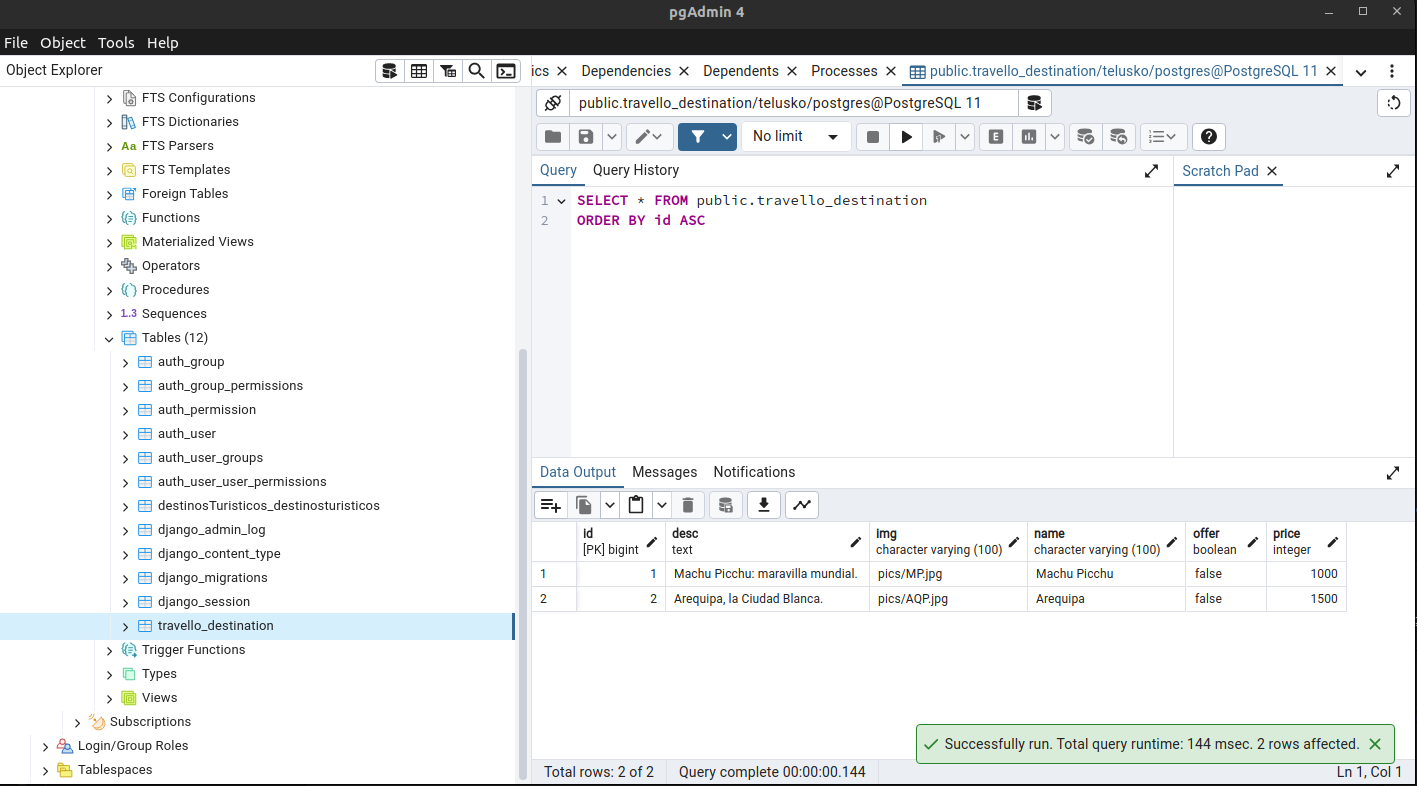
\includegraphics[width=0.7\textwidth]{img/travello-db.png}
  \caption{Codigo y Ejecucion}
\end{figure}

\section{DESTINOSTURISTICOS}

\section{Clases en Models.py}
El modelo DestinosTuristicos define los atributos necesarios para representar un destino turístico en una base de datos Django. Cada destino tiene un nombre de ciudad, una imagen asociada que se carga en la carpeta 'pics' del directorio de medios, una descripción textual, un precio para el tour y un indicador de oferta, que por defecto es 'False'. Este modelo proporciona una estructura coherente para almacenar información sobre destinos turísticos en una aplicación web Django.

\begin{figure}[H]
  \centering
  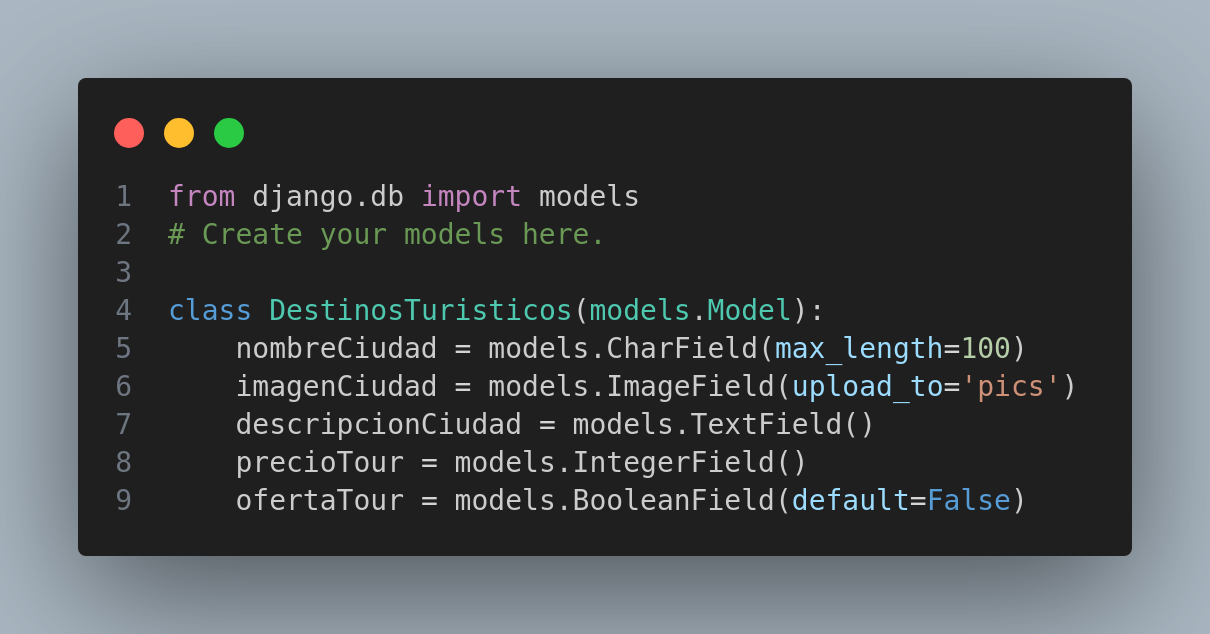
\includegraphics[width=0.7\textwidth]{img/models-DestinosTuristicos.png}
  \caption{Codigo y Ejecucion}
\end{figure}

\section{Funciones en Views.py}
Este conjunto de vistas en Django se encarga de gestionar las operaciones CRUD (Crear, Leer, Actualizar y Eliminar) para los destinos turísticos. La vista creardestino maneja la creación de nuevos destinos, listardestino muestra todos los destinos disponibles, editardestino permite modificar destinos existentes y eliminardestino facilita la eliminación de destinos. Cada vista procesa las solicitudes HTTP correspondientes, ya sea guardando datos nuevos, mostrando información existente o eliminando registros según lo especificado en la lógica de la aplicación.

\begin{figure}[H]
  \centering
  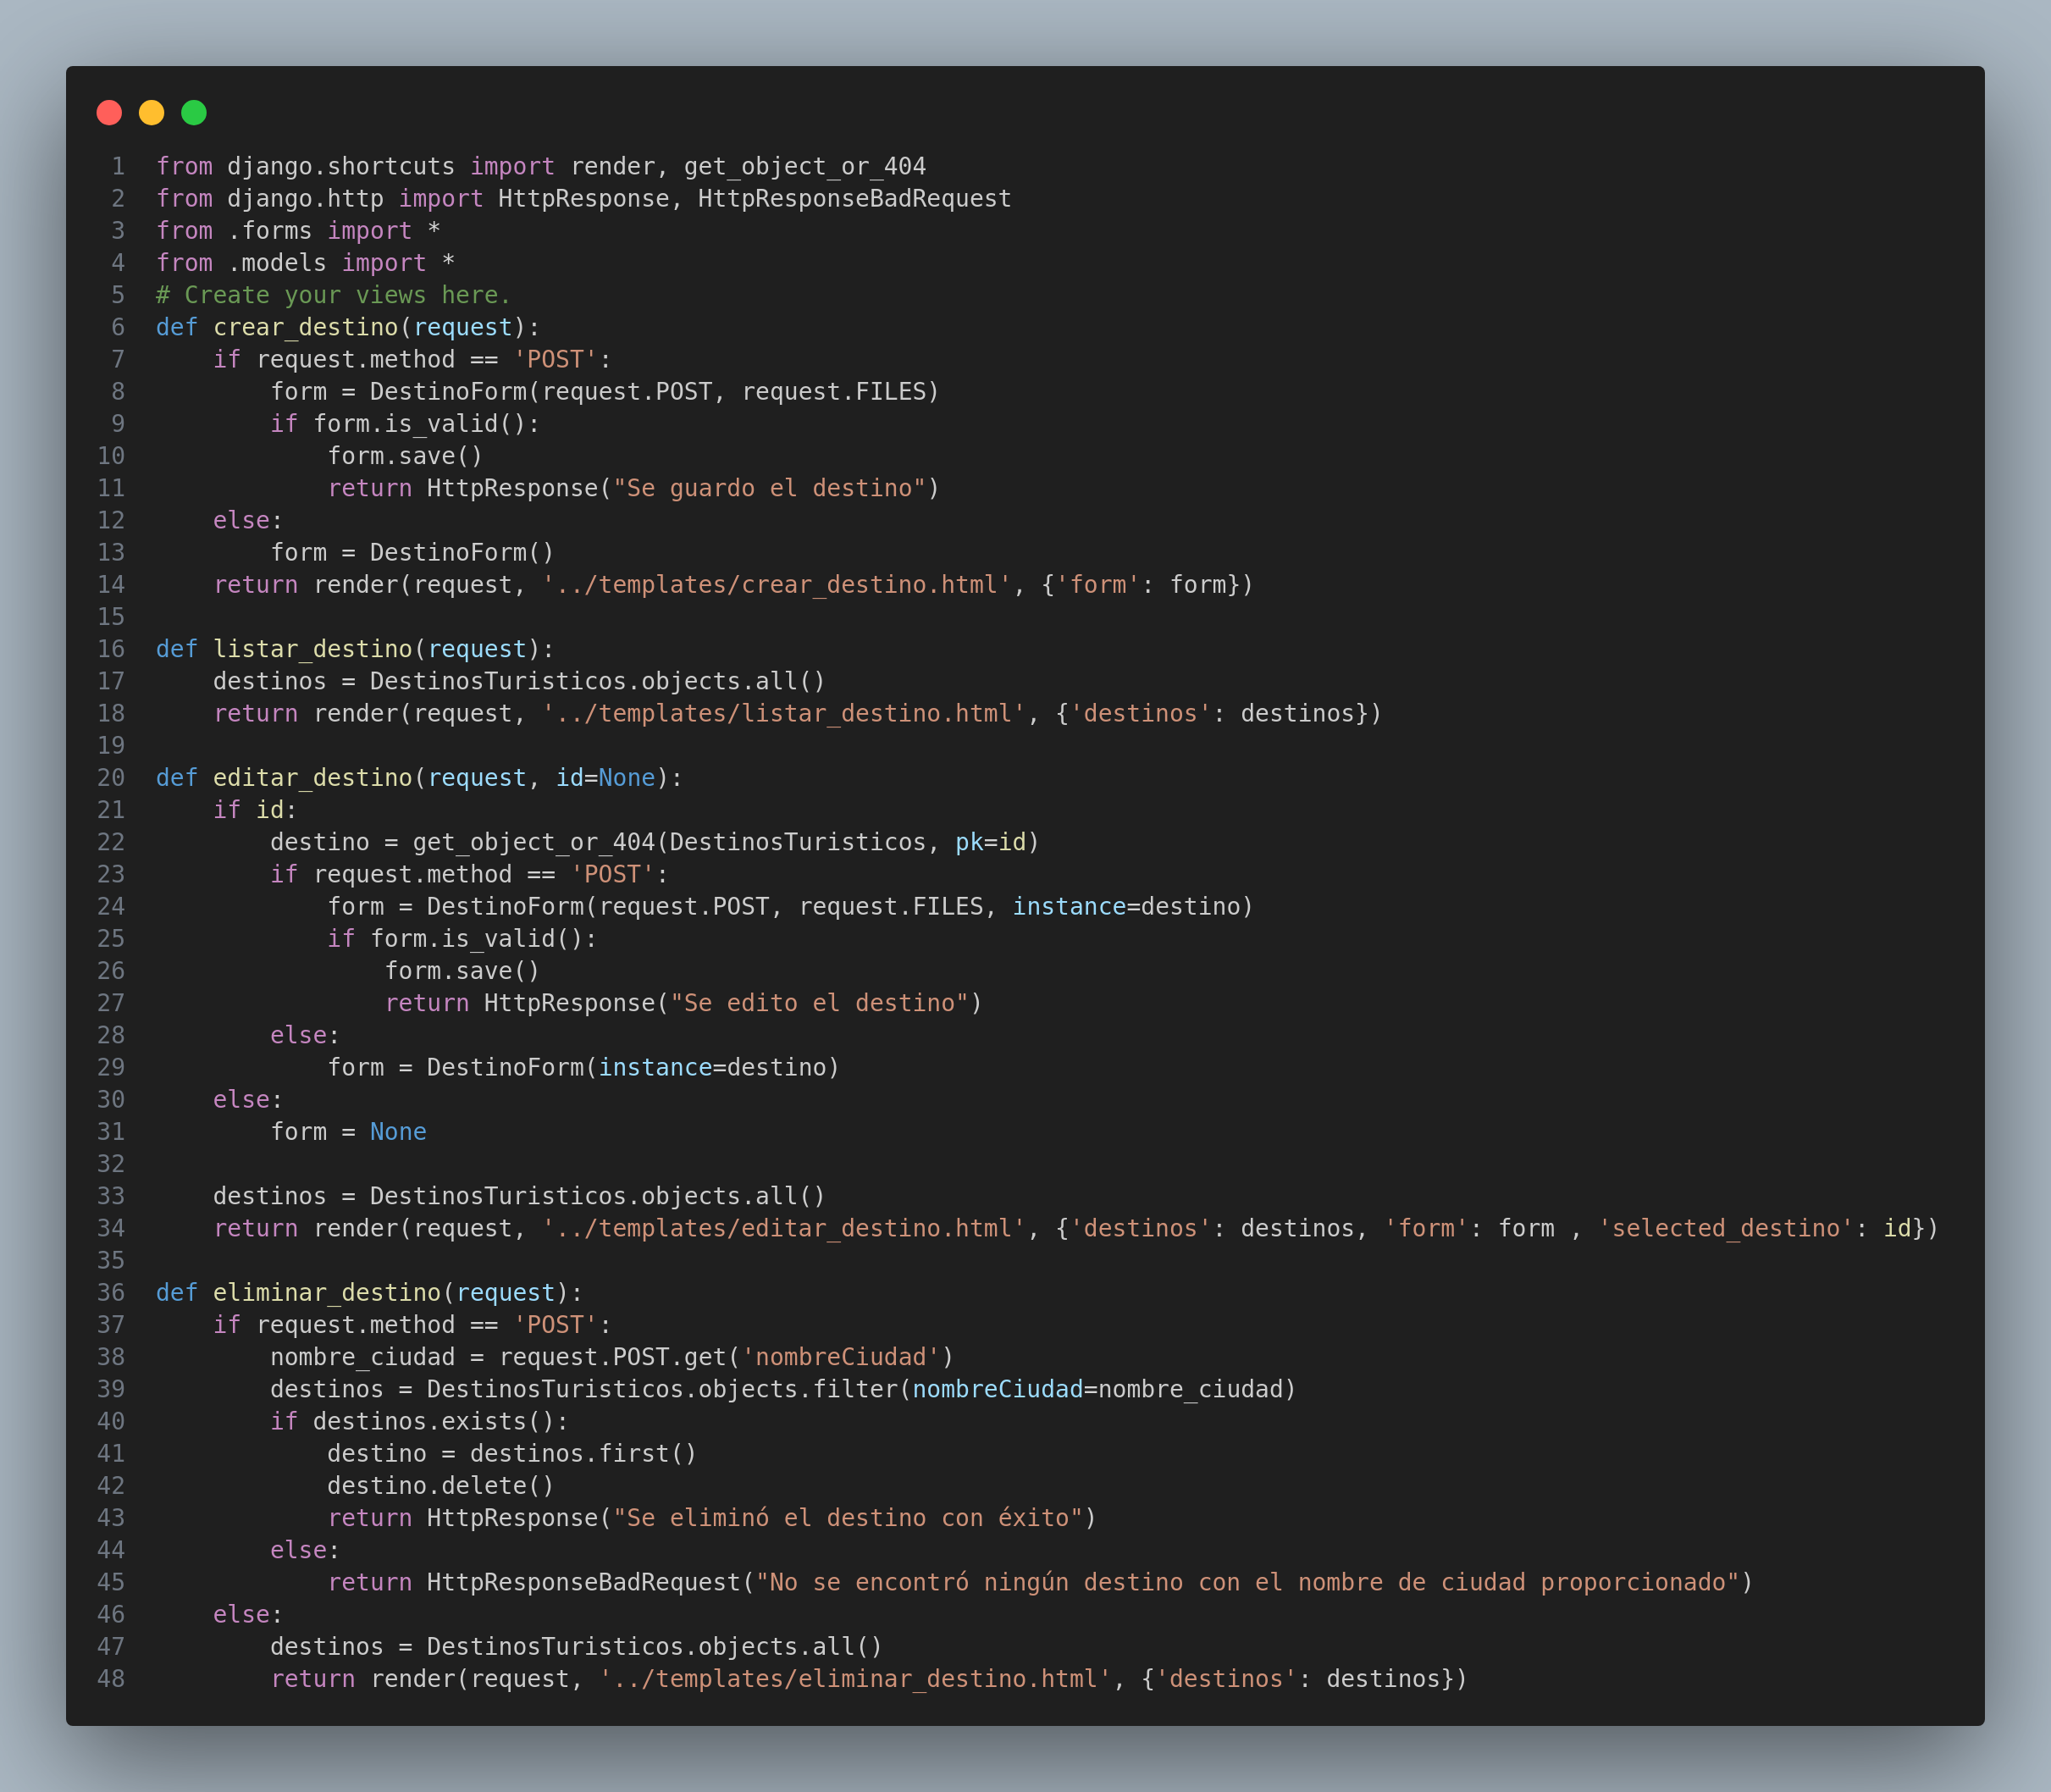
\includegraphics[width=0.7\textwidth]{img/views-DestinosTuristicos.png}
  \caption{Codigo y Ejecucion}
\end{figure}

\section{Funciones en Urls.py}
Estas son las URL configuradas para las vistas en la aplicación de destinos turísticos en Django. Cada URL está asociada a una función de vista específica. Por ejemplo, la URL crearDestino/ está vinculada a la vista creardestino, que maneja la creación de nuevos destinos. Además, hay una URL editarDestino/<int:id>/ que permite editar un destino específico identificado por su ID. Estas URL proporcionan puntos de acceso a las diferentes funcionalidades de la aplicación de destinos turísticos.

\begin{figure}[H]
  \centering
  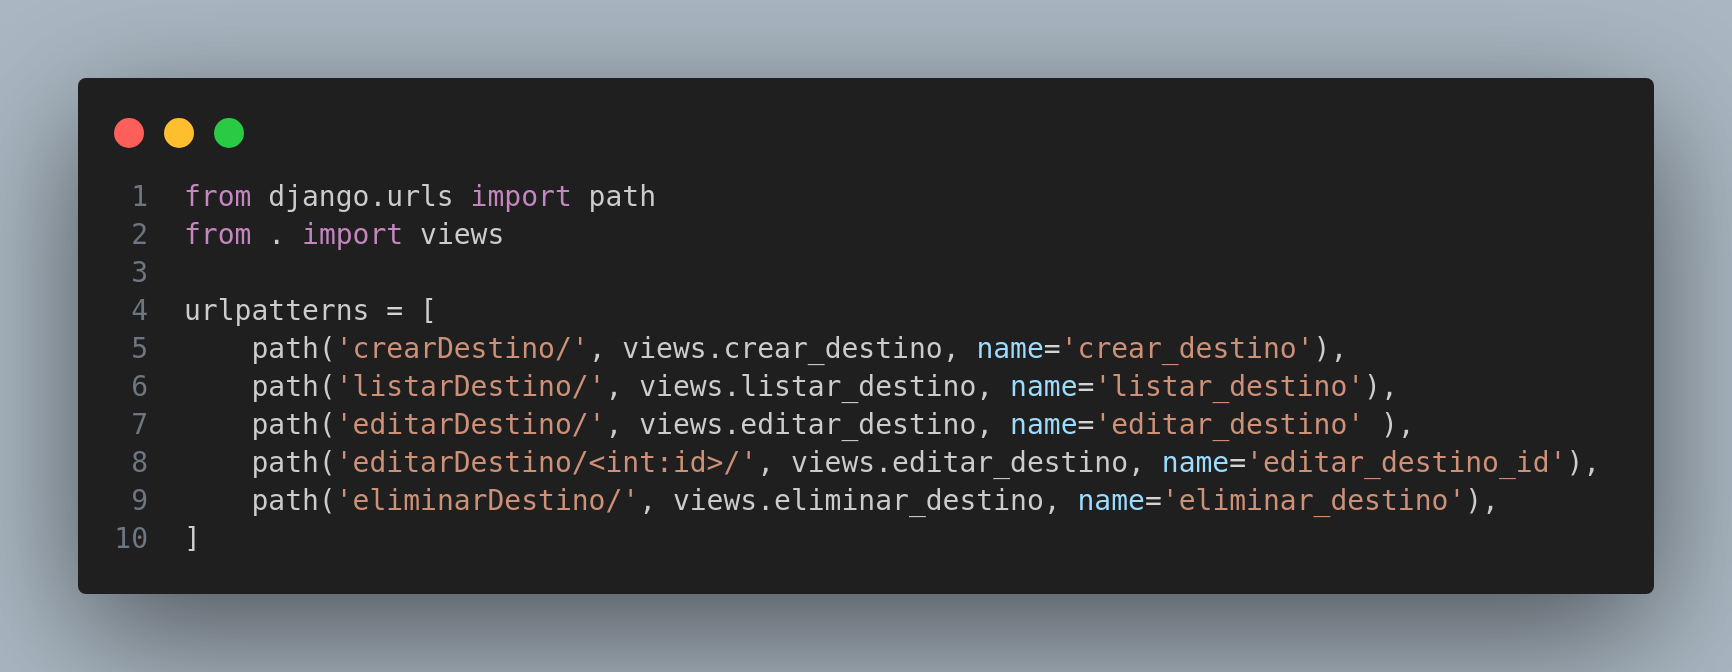
\includegraphics[width=0.7\textwidth]{img/urls-DestinosTuristicos.png}
  \caption{Codigo y Ejecucion}
\end{figure}

\section{Funciones en Forms.py}
El formulario DestinoForm se define utilizando la clase ModelForm de Django, que se importa del módulo django.forms. Este formulario está asociado al modelo DestinosTuristicos. Las propiedades del formulario coinciden con los campos del modelo, y se especifican en el atributo fields. Además, se ha definido un método save() personalizado para guardar los datos del formulario en la base de datos. Dentro de este método, se crea una instancia del modelo DestinosTuristicos con los datos del formulario y se guarda en la base de datos si commit es verdadero.

\begin{figure}[H]
  \centering
  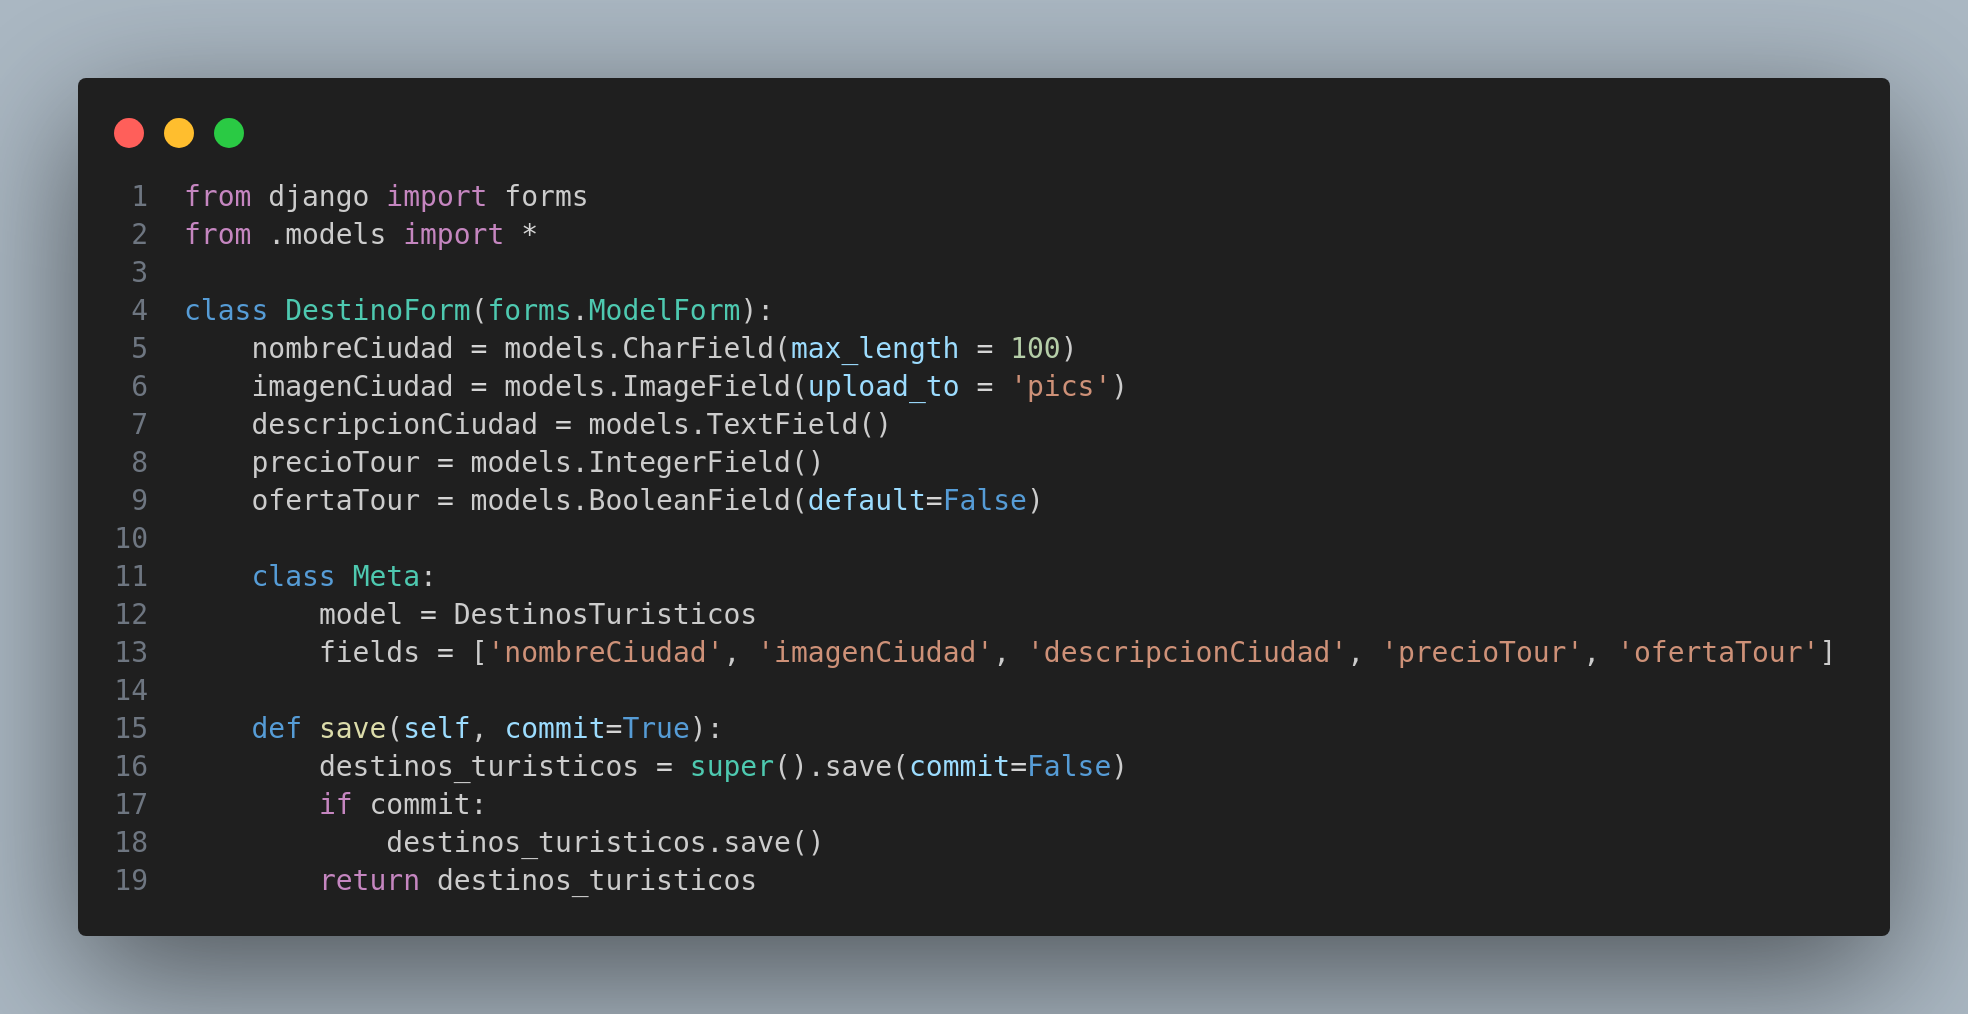
\includegraphics[width=0.7\textwidth]{img/forms-DestinosTuristicos.png}
  \caption{Codigo y Ejecucion}
\end{figure}

\section{Funciones en Admin.py}
Este fragmento de código Django importa la clase DestinosTuristicos del archivo models.py de la misma aplicación Django. Luego, registra esta clase en el panel de administración de Django utilizando admin.site.register(). Esto permite administrar los objetos de la clase DestinosTuristicos directamente desde el panel de administración de Django, lo que facilita la gestión de los datos relacionados con los destinos turísticos en la aplicación.

\begin{figure}[H]
  \centering
  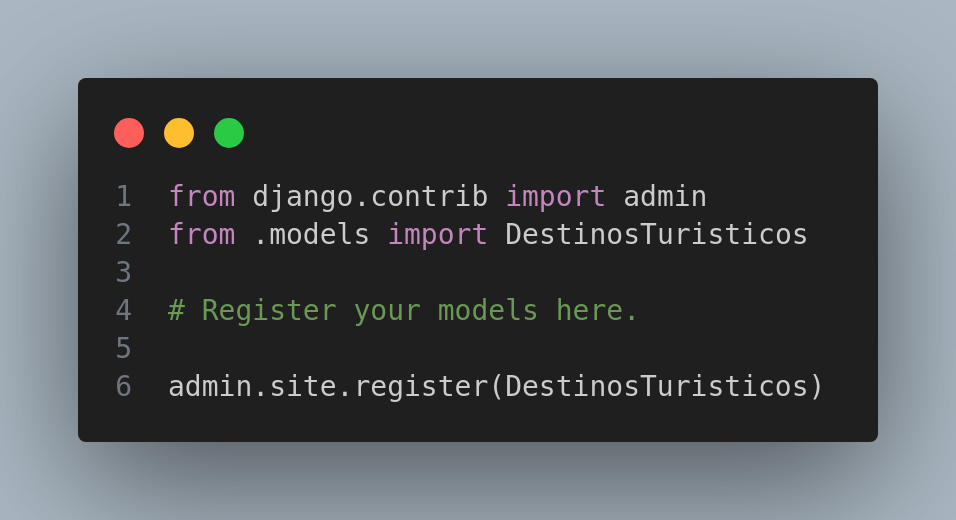
\includegraphics[width=0.7\textwidth]{img/admin-DestinosTuristicos.png}
  \caption{Codigo y Ejecucion}
\end{figure}

\section{Los archivos HTML}
Para poder visualizar el index nos ponemos en
travello \href{http://127.0.0.1:8000}{http://127.0.0.1:8000}

\begin{figure}[H]
  \centering
  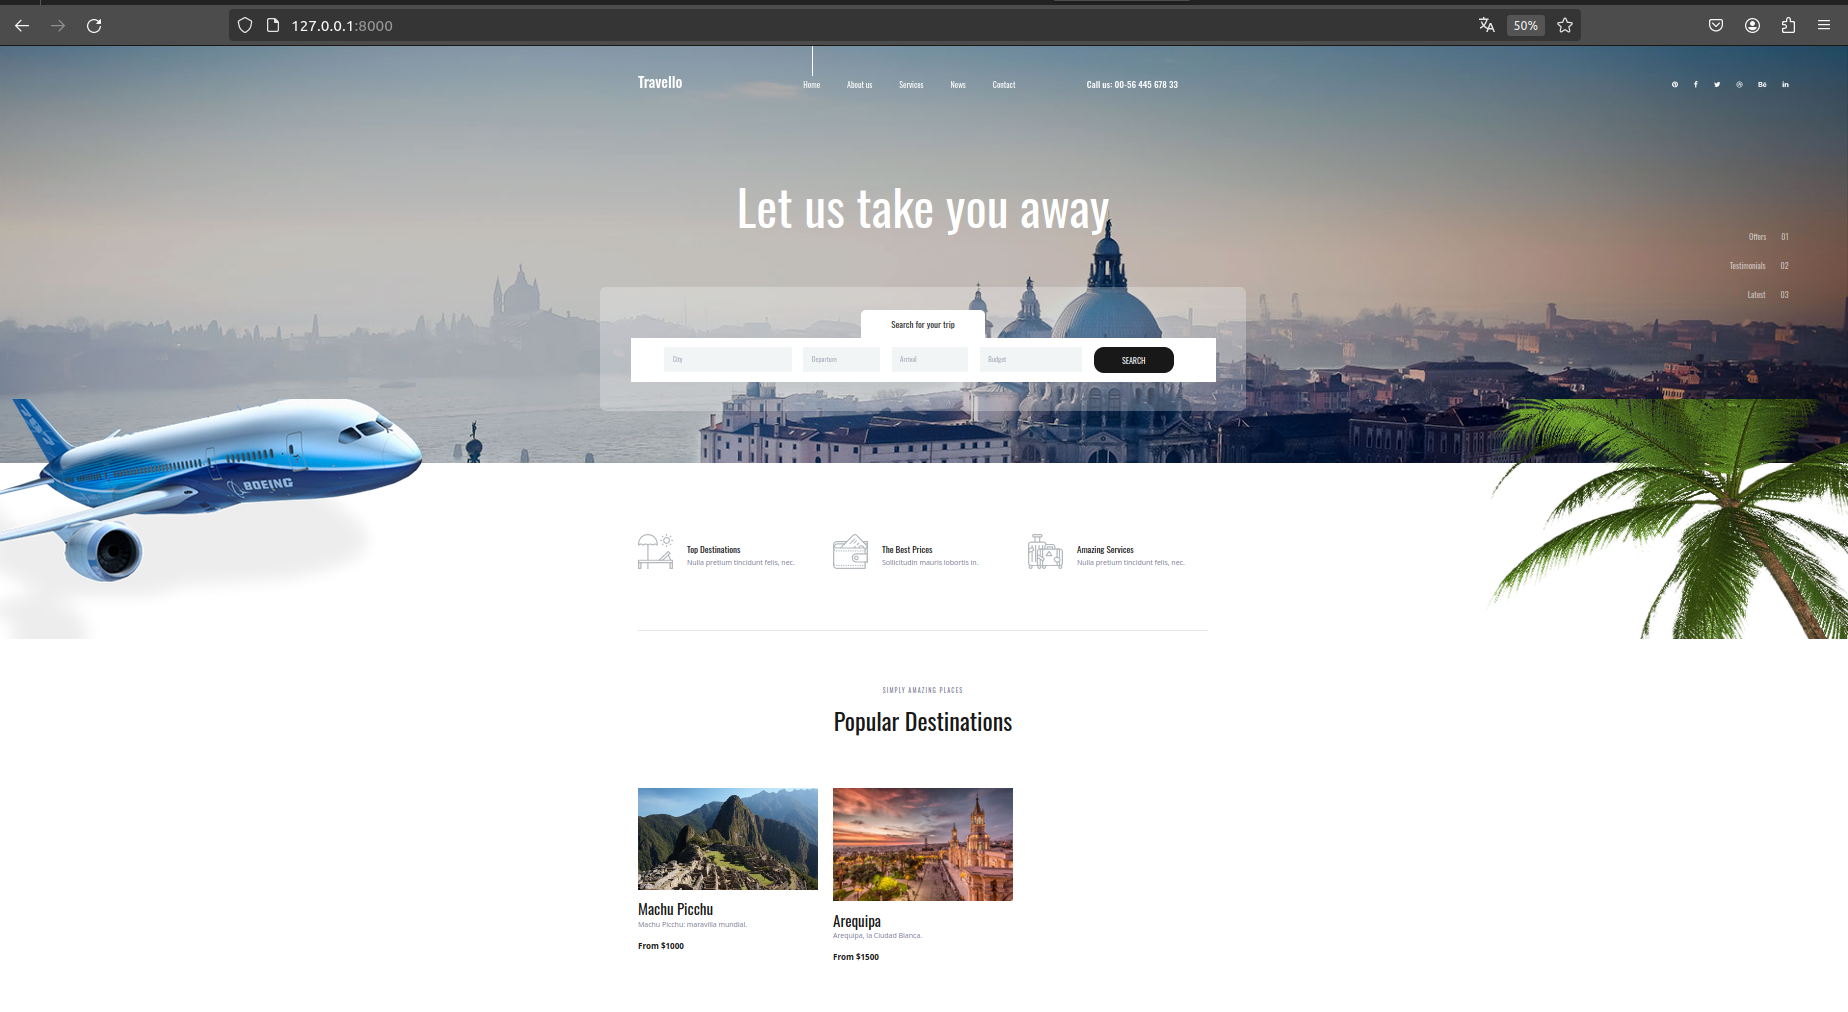
\includegraphics[width=0.7\textwidth]{img/index.png}
  \caption{Codigo y Ejecucion}
\end{figure}

Crear un destino en \href{http://127.0.0.1:8000/crearDestino/}{http://127.0.0.1:8000/crearDestino/}

\begin{figure}[H]
  \centering
  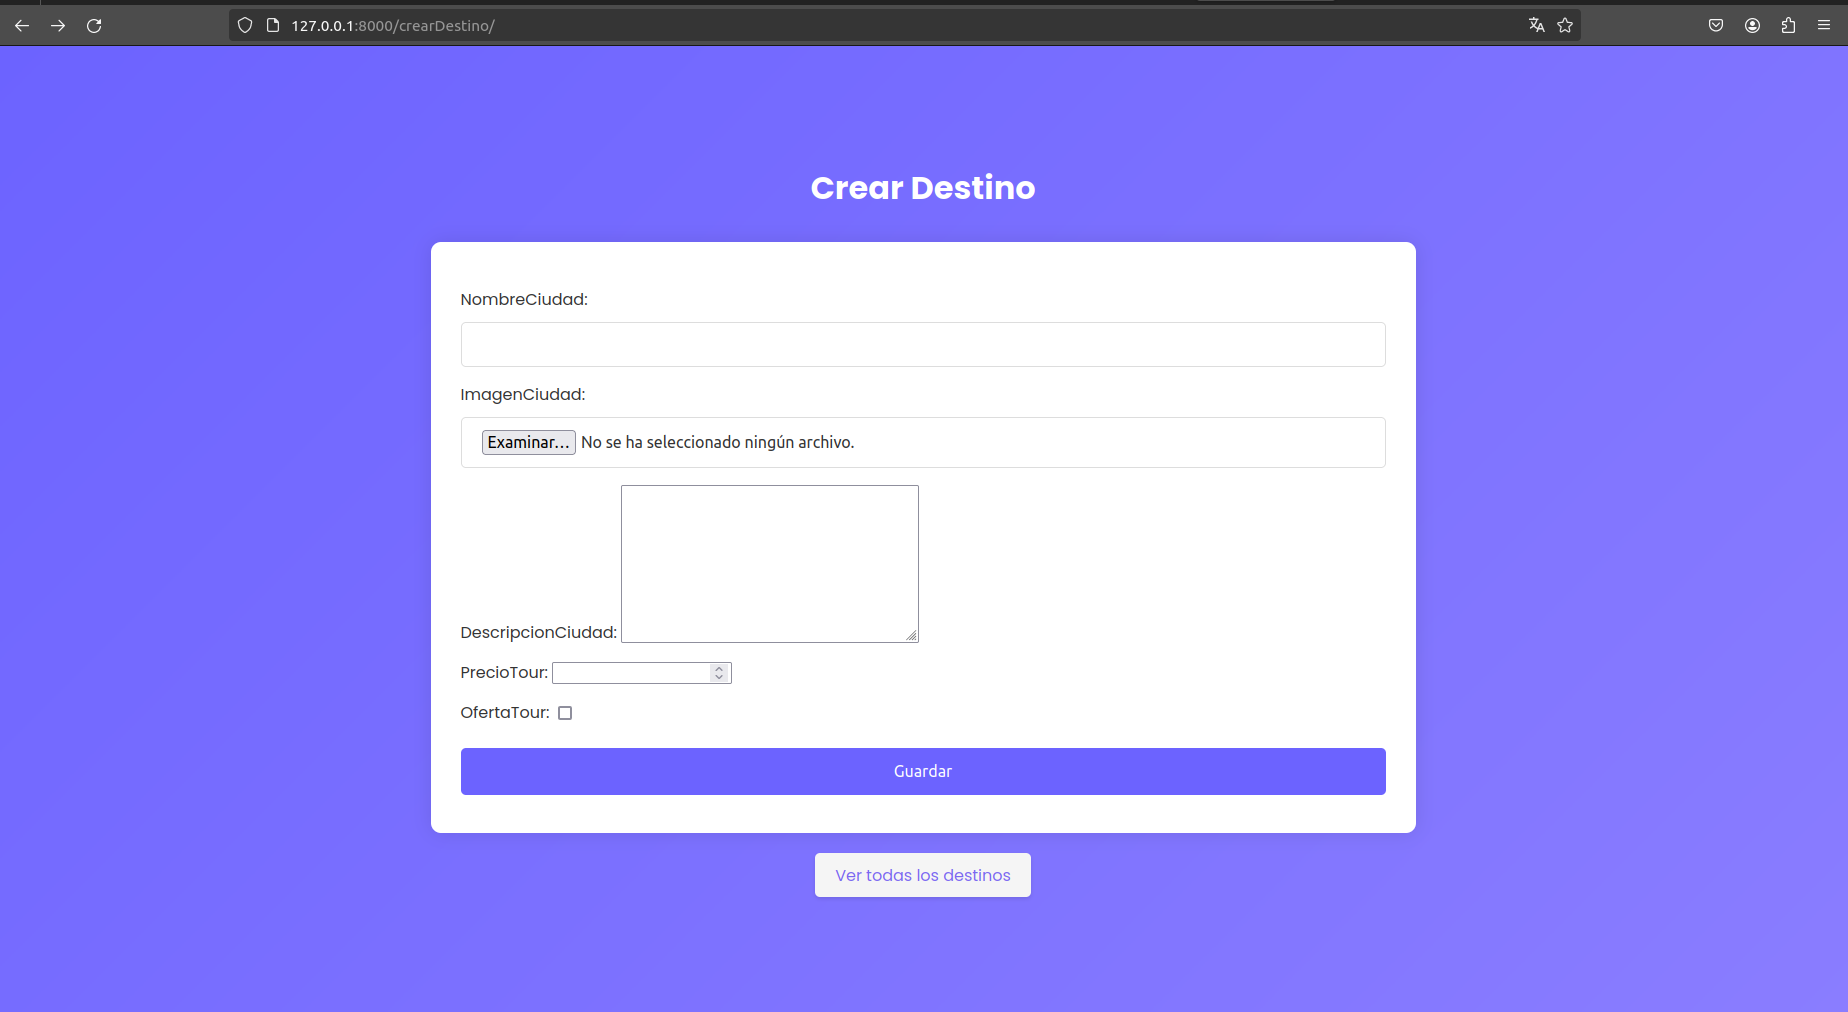
\includegraphics[width=0.7\textwidth]{img/crear.png}
  \caption{Codigo y Ejecucion}
\end{figure}

\singlespacing
Listar destinos en \href{http://127.0.0.1:8000/listarDestino/}{http://127.0.0.1:8000/listarDestino/}

\begin{figure}[H]
  \centering
  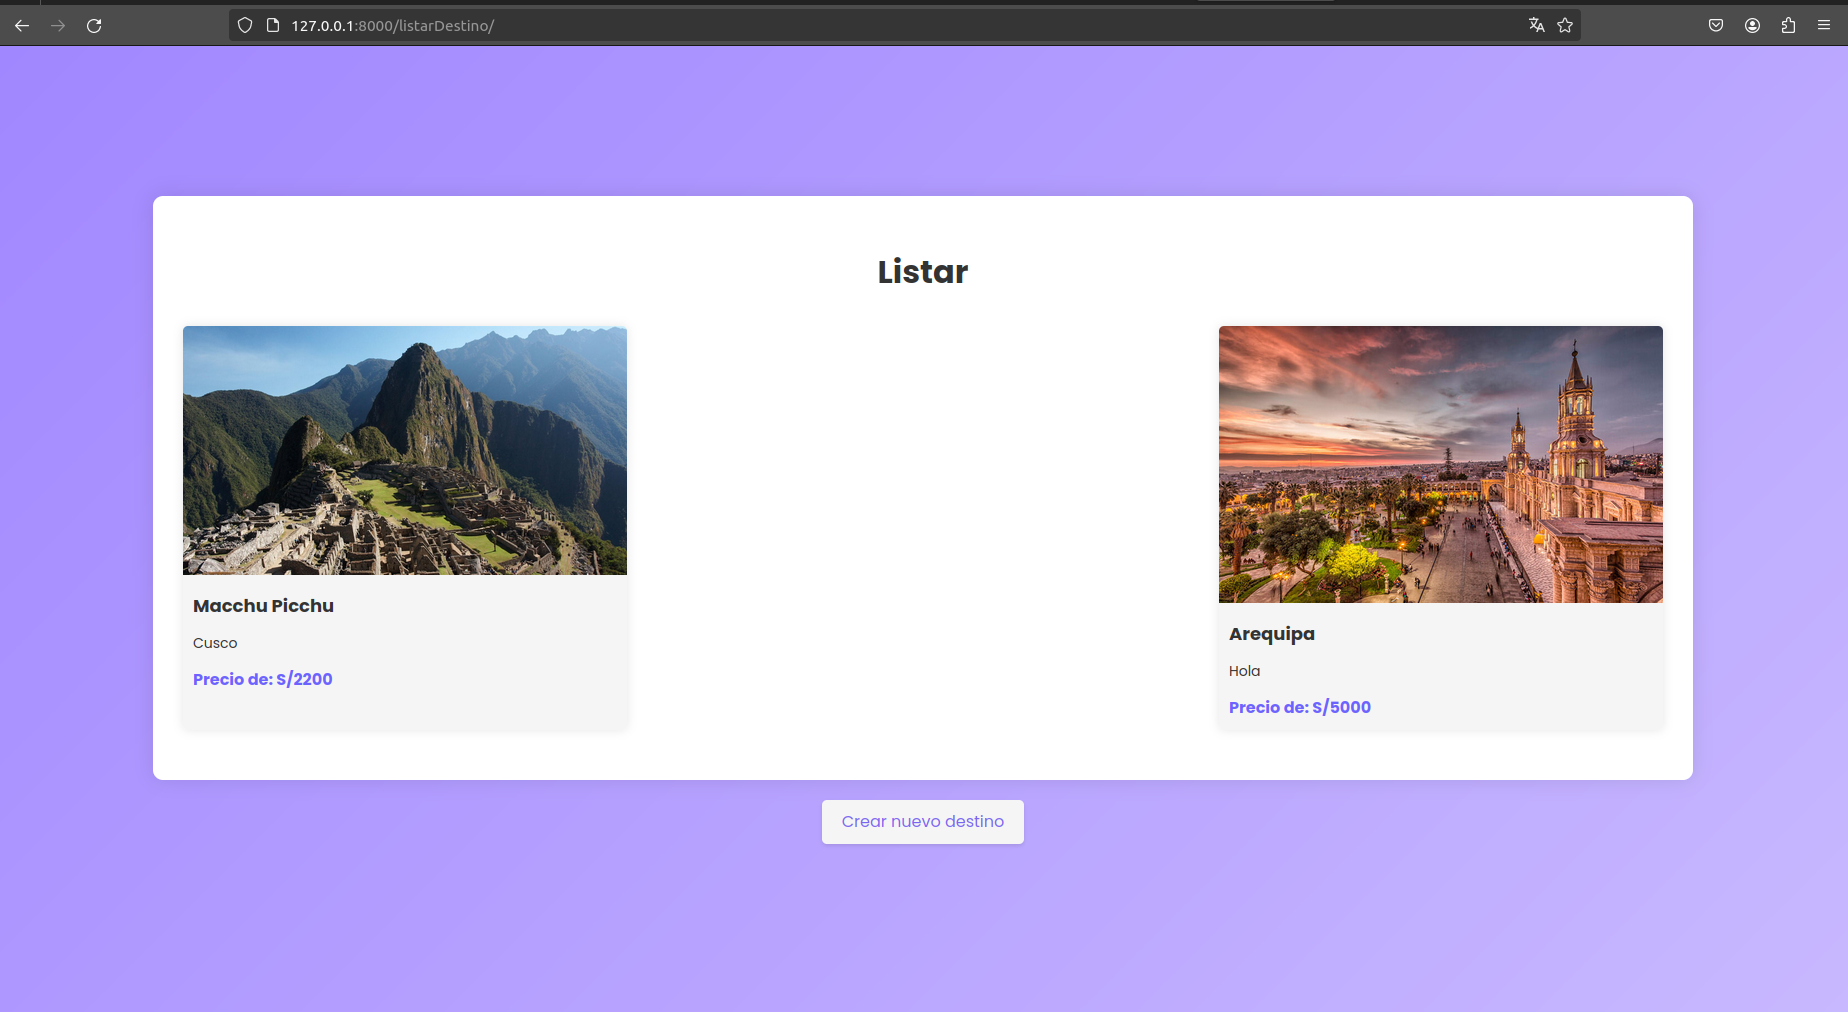
\includegraphics[width=0.7\textwidth]{img/listar.png}
  \caption{Codigo y Ejecucion}
\end{figure}

\singlespacing
Editar un destino en \href{http://127.0.0.1:8000/editarDestino/}{http://127.0.0.1:8000/editarDestino/}

\begin{figure}[H]
  \centering
  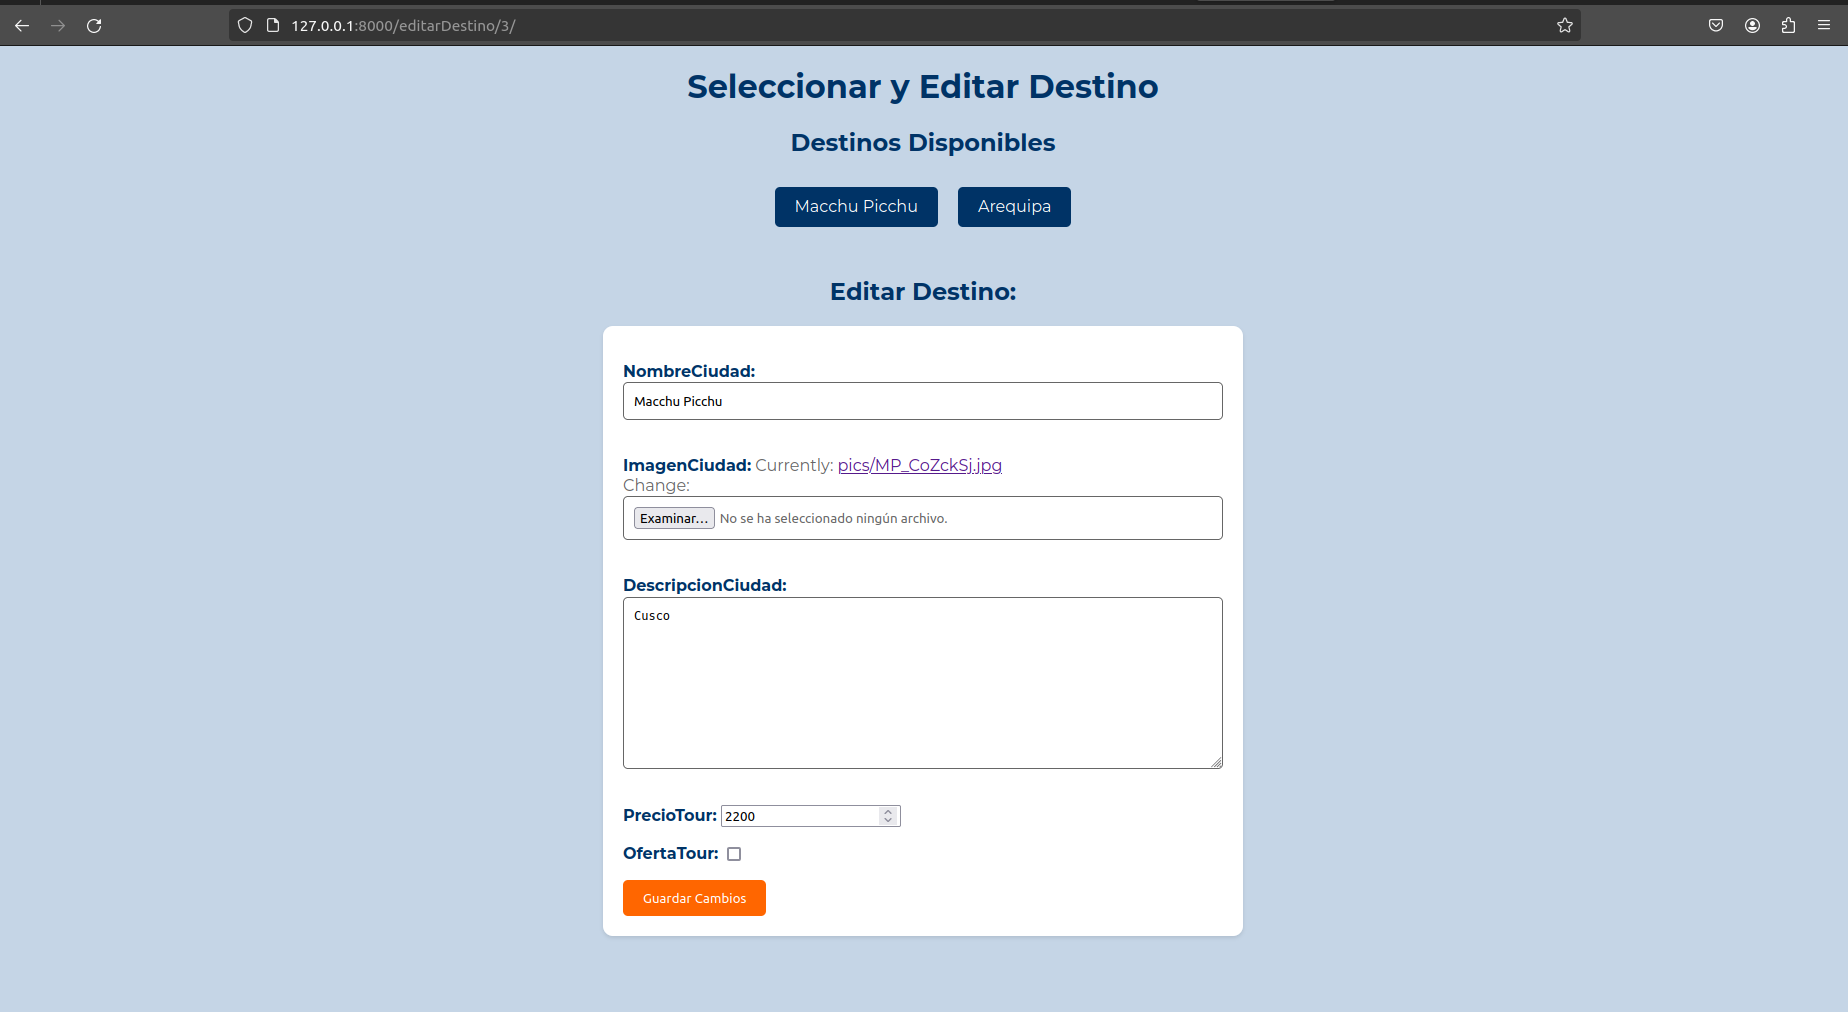
\includegraphics[width=0.7\textwidth]{img/editar.png}
  \caption{Codigo y Ejecucion}
\end{figure}

\singlespacing
Eliminar un destino en \href{http://127.0.0.1:8000/eliminarDestino/}{http://127.0.0.1:8000/eliminarDestino/}

\begin{figure}[H]
  \centering
  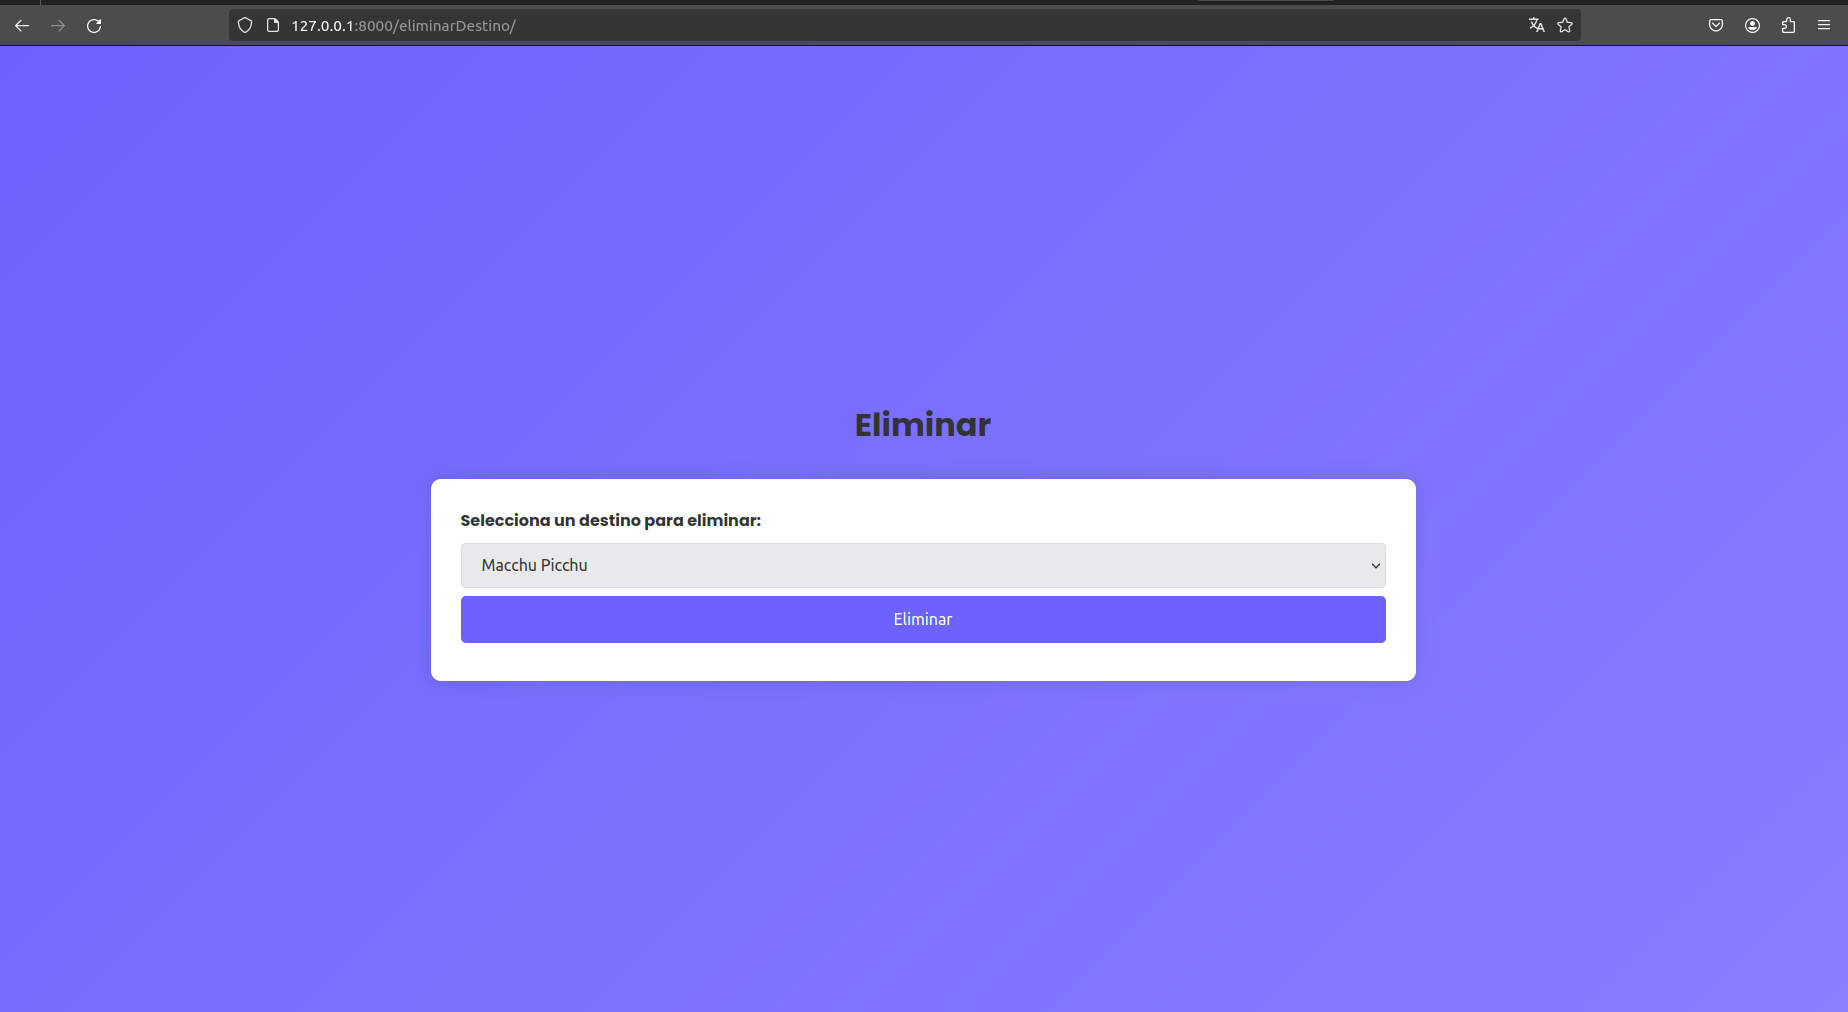
\includegraphics[width=0.7\textwidth]{img/eliminar.png}
  \caption{Codigo y Ejecucion}
\end{figure}

\section{Base de Datos PostgradeSQL}

\section{Entrar a Django Admin}
Crear un destino en \href{http://127.0.0.1:8000/admin/login/?next=/admin/}{http://127.0.0.1:8000/admin/login/?next=/admin/}
\singlespacing
Cuando entremos hay que crear un superusuario para el admin y poder administrar la base de datos para esto hay crearlo desde la terminal

\begin{figure}[H]
  \centering
  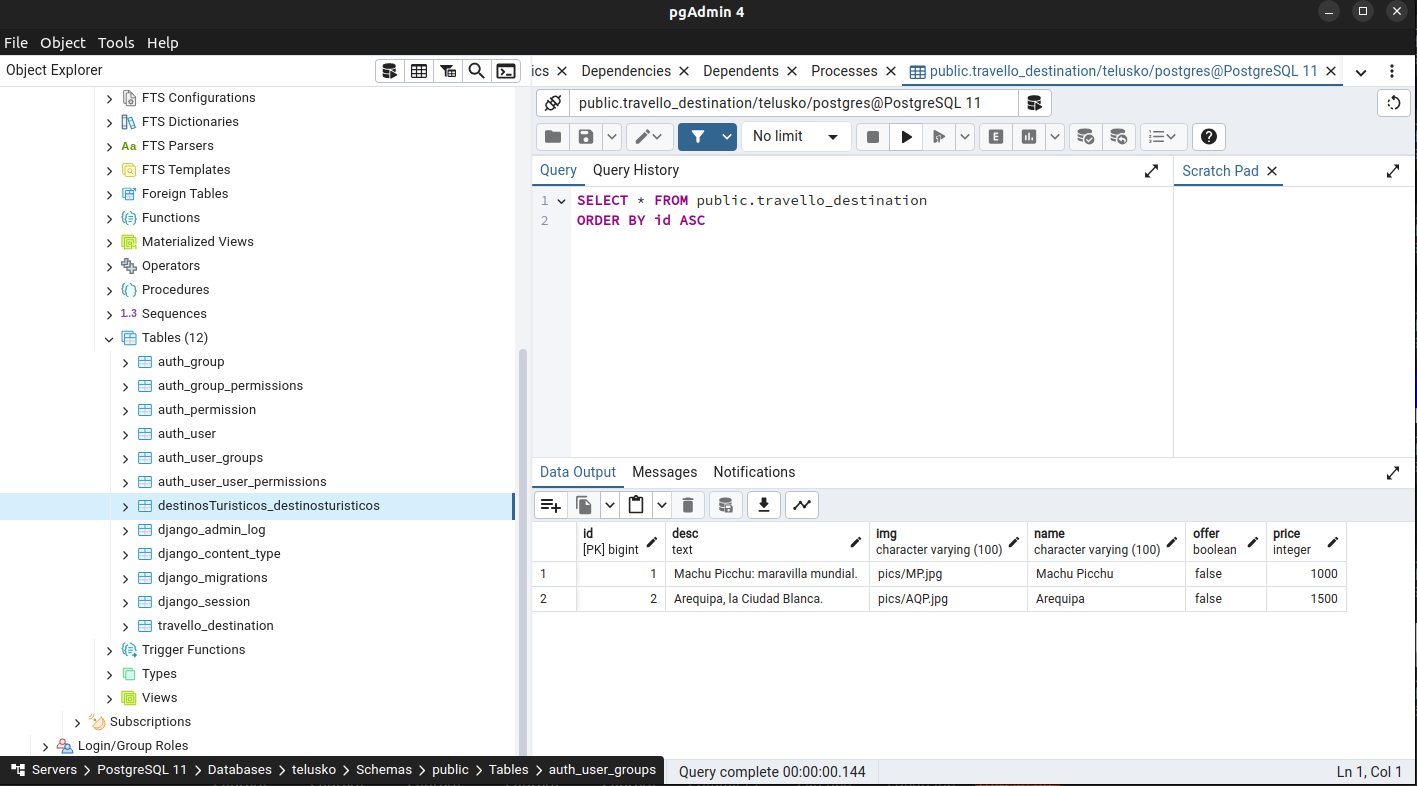
\includegraphics[width=0.7\textwidth]{img/destinos-db.png}
  \caption{Codigo y Ejecucion}
\end{figure}

\section{El proyecto es cual es TELUSKO}
\section{Funciones en Urls.py en el proyecto}
Este archivo configura las URL para el proyecto telusko. El patrón de URL vacío ('') está incluido para las aplicaciones travello y destinosTuristicos, lo que significa que las URL definidas en los archivos urls.py de esas aplicaciones estarán disponibles en la raíz del sitio. Además, se incluye la URL para el panel de administración de Django en admin/.


\begin{figure}[H]
  \centering
  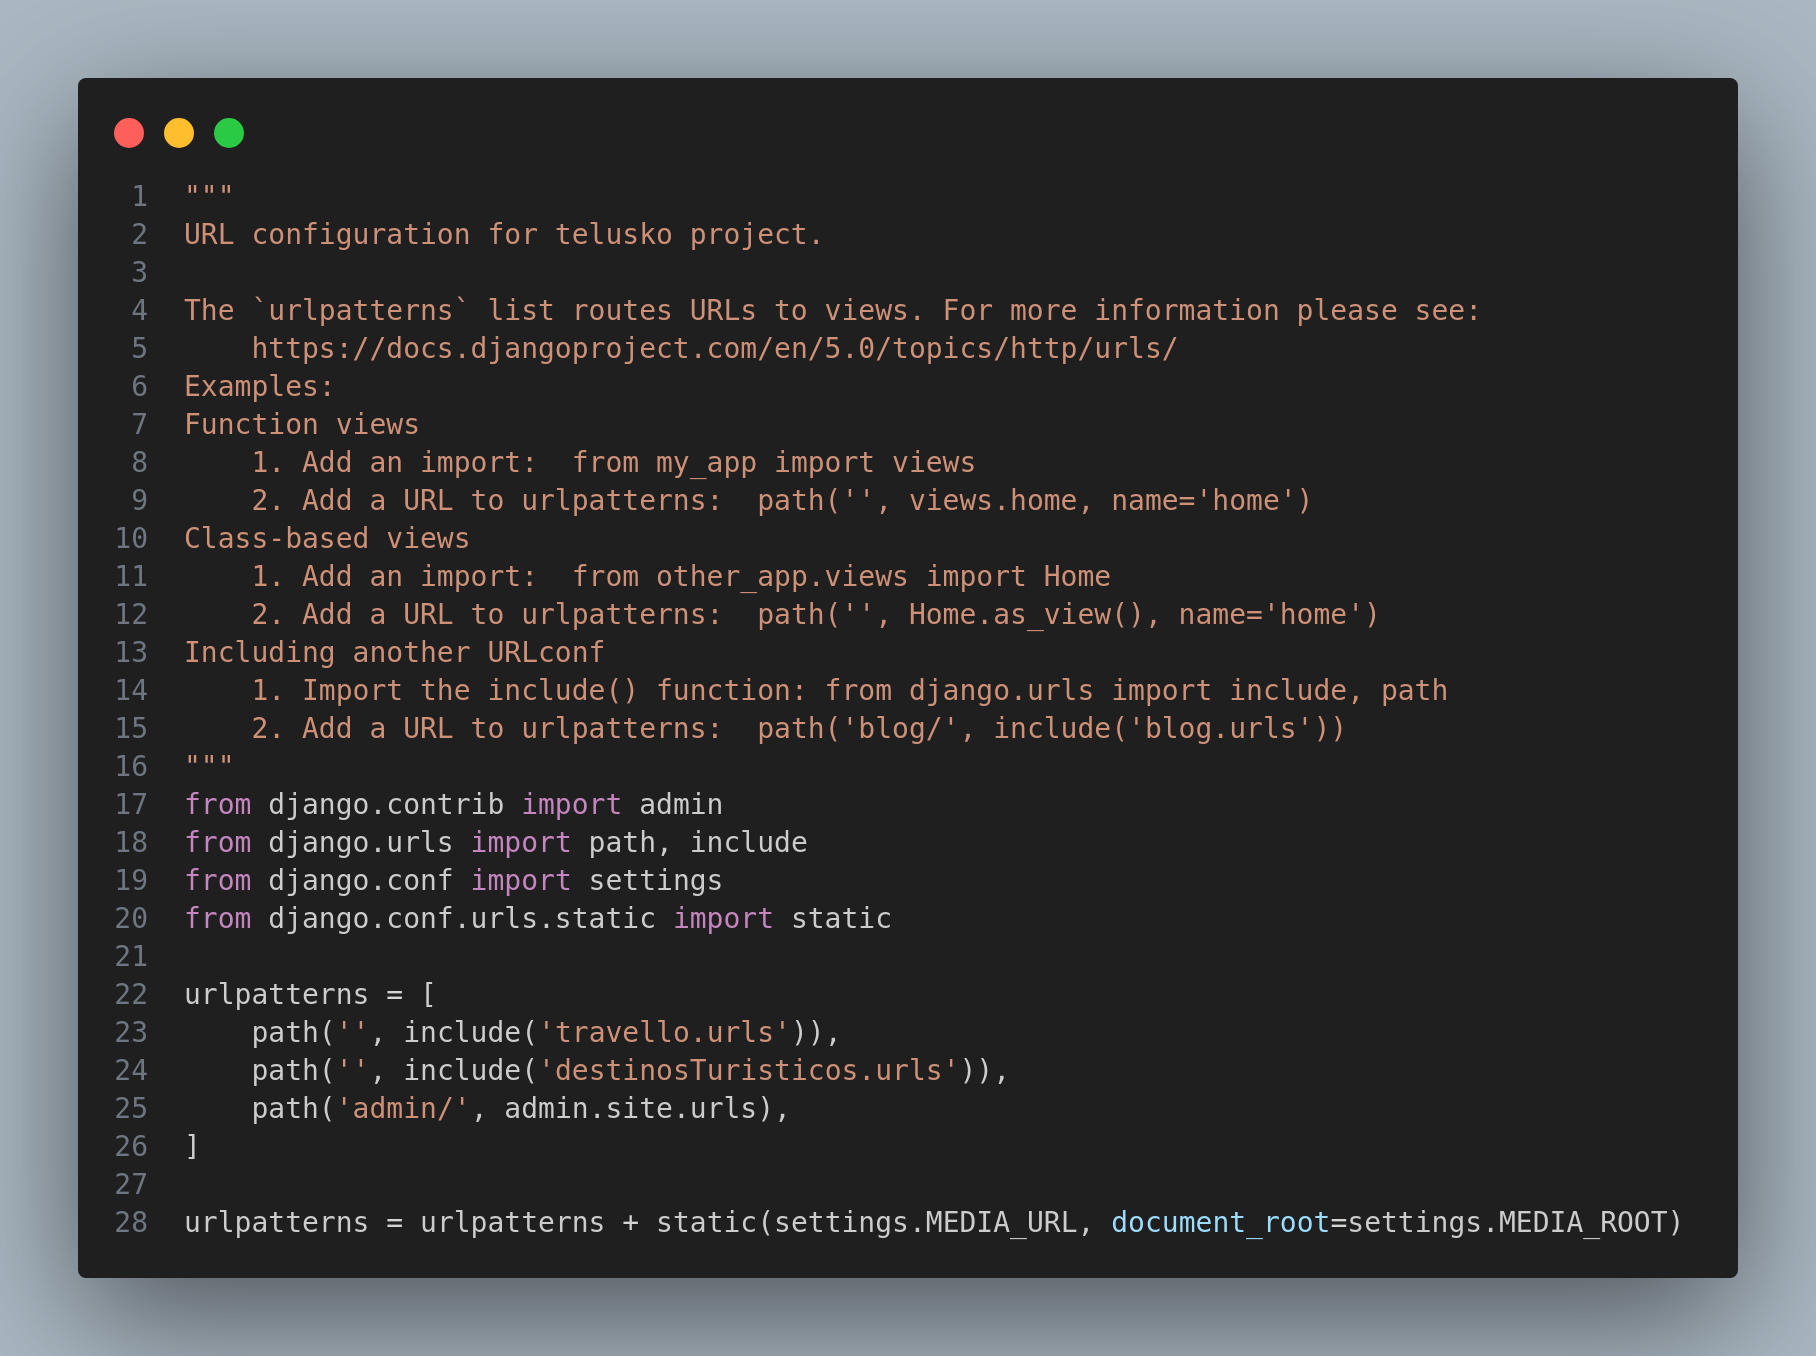
\includegraphics[width=0.7\textwidth]{img/urls-telusko.png}
  \caption{Codigo y Ejecucion}
\end{figure}

\singlespacing
Además, se agrega la configuración para servir archivos multimedia en desarrollo, agregando las URL MEDIA-URL y MEDIAROOT definidas en la configuración de Django. Esto permite que los archivos multimedia, como imágenes cargadas, se sirvan correctamente durante el desarrollo del proyecto.
\section{Funciones en Settings.py}
El fragmento proporcionado configura las aplicaciones y la conexión a la base de datos en un proyecto Django. En la lista INSTALLED/APPS, se enumeran las aplicaciones instaladas, incluidas las específicas del proyecto (destinosTuristicos y travello) y las aplicaciones predeterminadas de Django para funcionalidades como la administración, la autenticación y el manejo de sesiones. Por otro lado, en la sección DATABASES, se define la configuración para conectarse a una base de datos PostgreSQL, especificando el nombre de la base de datos, el nombre de usuario, la contraseña y el host. Estos elementos son esenciales para establecer el entorno de desarrollo y la infraestructura de almacenamiento de datos para el proyecto Django.
\begin{figure}[H]
  \centering
  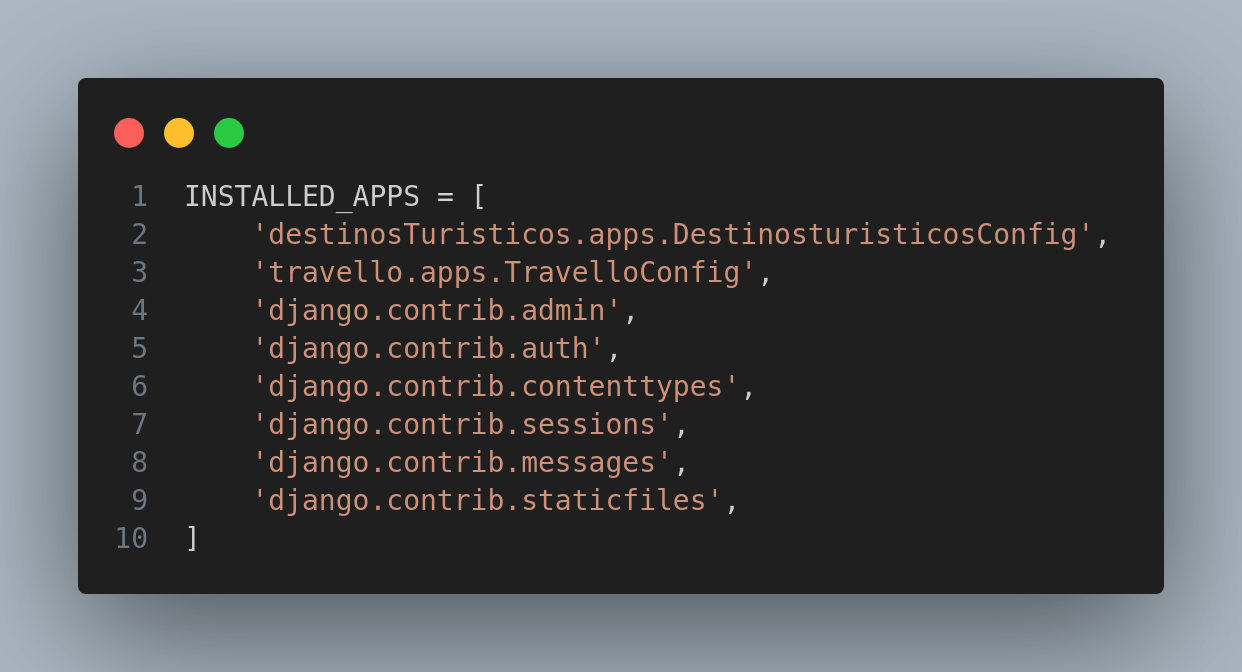
\includegraphics[width=0.7\textwidth]{img/settings-app-telusko.png}
  \caption{Codigo y Ejecucion}
\end{figure}

\begin{figure}[H]
  \centering
  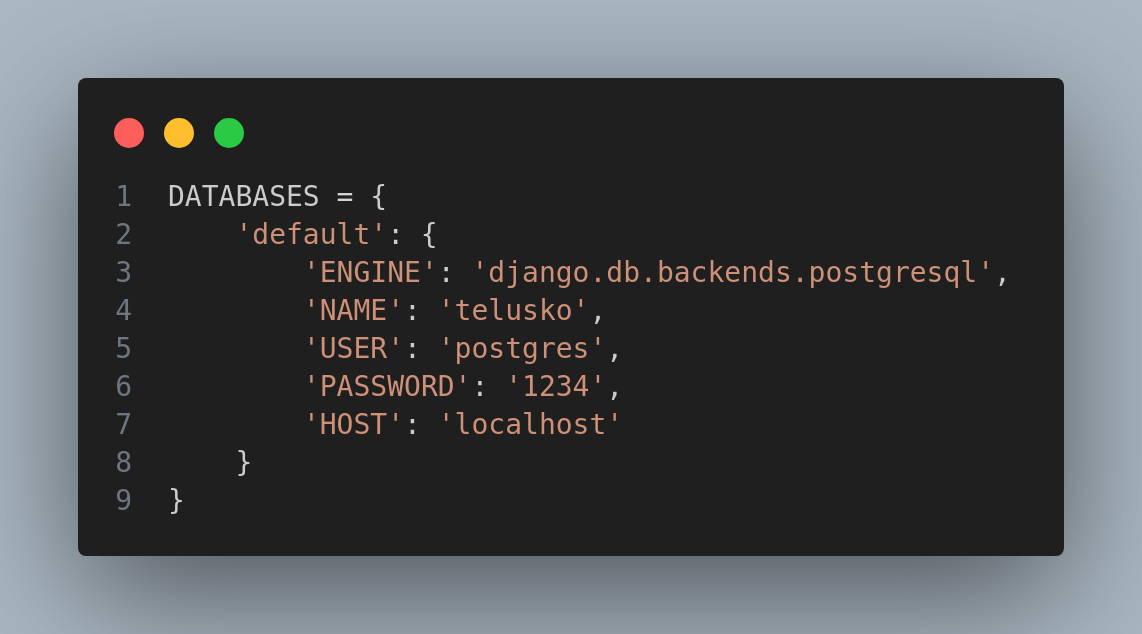
\includegraphics[width=0.7\textwidth]{img/settings-db-telusko.png}
  \caption{Codigo y Ejecucion}
\end{figure}



\section{Ejecutar el servidor}
El comando python manage.py makemigrations colegio se utiliza en Django para crear nuevas migraciones basadas en los cambios realizados en los modelos del aplicativo colegio. Las migraciones son archivos que describen cómo modificar la estructura de la base de datos para mantenerla sincronizada con los modelos de Django. Este comando analiza los modelos en la aplicación colegio y genera los archivos de migración necesarios para aplicar esos cambios a la base de datos.
\begin{lstlisting}[language=bash]
  python manage.py makemigrations travello
  python3 manage.py sqlmigrate travello 0001
  python3 manage.py sqlmigrate travello 0002
  python manage.py makemigrations destinosTuristicos
  python manage.py sqlmigrate destinosTuristicos 0001
  python manage.py migrate
\end{lstlisting}

El comando python manage.py runserver se utiliza en Django para iniciar el servidor de desarrollo local. Una vez ejecutado, el servidor se activa y permite acceder a la aplicación web en desarrollo a través de un navegador en la dirección http://localhost:8000/ por defecto. Es una herramienta fundamental durante el proceso de desarrollo de aplicaciones web con Django, ya que proporciona un entorno de prueba para probar y depurar el código antes de desplegar la aplicación en un entorno de producción.
\begin{lstlisting}[language=bash]
  python manage.py runserver
\end{lstlisting}

\section{Acceder a la aplicacion en el navegador}
travello \href{http://127.0.0.1:8000}{http://127.0.0.1:8000}
\singlespacing
Crear un destino en \href{http://127.0.0.1:8000/crearDestino/}{http://127.0.0.1:8000/crearDestino/}
\singlespacing
Listar destinos en \href{http://127.0.0.1:8000/listarDestino/}{http://127.0.0.1:8000/listarDestino/}
\singlespacing
Editar un destino en \href{http://127.0.0.1:8000/editarDestino/}{http://127.0.0.1:8000/editarDestino/}
\singlespacing
Eliminar un destino en \href{http://127.0.0.1:8000/eliminarDestino/}{http://127.0.0.1:8000/eliminarDestino/}

\section{Flip}
No carga mi video en flip por ellos use un link de drive
\begin{figure}[H]
  \centering
  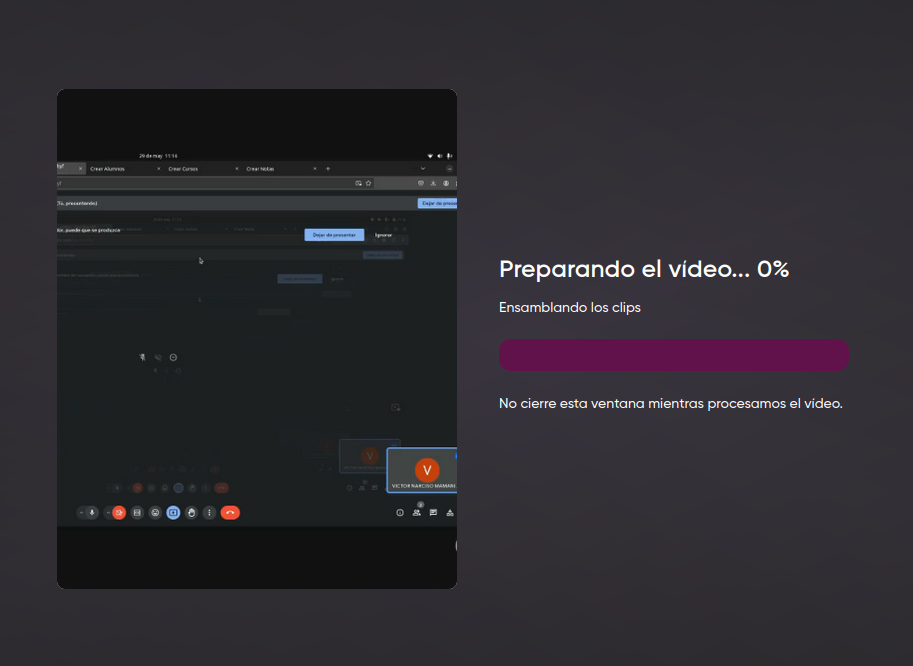
\includegraphics[width=0.7\textwidth]{img/Flip.png}
  \caption{Codigo y Ejecucion}
\end{figure}


\end{figure}
\item \textbf{URL de video de explicación:} \url{}
\item \textbf{URL de repositorio de GitHub:} \url{https://github.com/VictorMA18/Lab07-Django-Telusko}
\end{document}


